
%% bare_conf.tex
%% V1.4b
%% 2015/08/26
%% by Michael Shell
%% See:
%% http://www.michaelshell.org/
%% for current contact information.
%%
%% This is a skeleton file demonstrating the use of IEEEtran.cls
%% (requires IEEEtran.cls version 1.8b or later) with an IEEE
%% conference paper.
%%
%% Support sites:
%% http://www.michaelshell.org/tex/ieeetran/
%% http://www.ctan.org/pkg/ieeetran
%% and
%% http://www.ieee.org/

%%*************************************************************************
%% Legal Notice:
%% This code is offered as-is without any warranty either expressed or
%% implied; without even the implied warranty of MERCHANTABILITY or
%% FITNESS FOR A PARTICULAR PURPOSE! 
%% User assumes all risk.
%% In no event shall the IEEE or any contributor to this code be liable for
%% any damages or losses, including, but not limited to, incidental,
%% consequential, or any other damages, resulting from the use or misuse
%% of any information contained here.
%%
%% All comments are the opinions of their respective authors and are not
%% necessarily endorsed by the IEEE.
%%
%% This work is distributed under the LaTeX Project Public License (LPPL)
%% ( http://www.latex-project.org/ ) version 1.3, and may be freely used,
%% distributed and modified. A copy of the LPPL, version 1.3, is included
%% in the base LaTeX documentation of all distributions of LaTeX released
%% 2003/12/01 or later.
%% Retain all contribution notices and credits.
%% ** Modified files should be clearly indicated as such, including  **
%% ** renaming them and changing author support contact information. **
%%*************************************************************************


% *** Authors should verify (and, if needed, correct) their LaTeX system  ***
% *** with the testflow diagnostic prior to trusting their LaTeX platform ***
% *** with production work. The IEEE's font choices and paper sizes can   ***
% *** trigger bugs that do not appear when using other class files.       ***                          ***
% The testflow support page is at:
% http://www.michaelshell.org/tex/testflow/



\documentclass[conference]{IEEEtran}
% Some Computer Society conferences also require the compsoc mode option,
% but others use the standard conference format.
%
% If IEEEtran.cls has not been installed into the LaTeX system files,
% manually specify the path to it like:
% \documentclass[conference]{../sty/IEEEtran}





% Some very useful LaTeX packages include:
% (uncomment the ones you want to load)


% *** MISC UTILITY PACKAGES ***
%
%\usepackage{ifpdf}
% Heiko Oberdiek's ifpdf.sty is very useful if you need conditional
% compilation based on whether the output is pdf or dvi.
% usage:
% \ifpdf
%   % pdf code
% \else
%   % dvi code
% \fi
% The latest version of ifpdf.sty can be obtained from:
% http://www.ctan.org/pkg/ifpdf
% Also, note that IEEEtran.cls V1.7 and later provides a builtin
% \ifCLASSINFOpdf conditional that works the same way.
% When switching from latex to pdflatex and vice-versa, the compiler may
% have to be run twice to clear warning/error messages.






% *** CITATION PACKAGES ***
%
%\usepackage{cite}
% cite.sty was written by Donald Arseneau
% V1.6 and later of IEEEtran pre-defines the format of the cite.sty package
% \cite{} output to follow that of the IEEE. Loading the cite package will
% result in citation numbers being automatically sorted and properly
% "compressed/ranged". e.g., [1], [9], [2], [7], [5], [6] without using
% cite.sty will become [1], [2], [5]--[7], [9] using cite.sty. cite.sty's
% \cite will automatically add leading space, if needed. Use cite.sty's
% noadjust option (cite.sty V3.8 and later) if you want to turn this off
% such as if a citation ever needs to be enclosed in parenthesis.
% cite.sty is already installed on most LaTeX systems. Be sure and use
% version 5.0 (2009-03-20) and later if using hyperref.sty.
% The latest version can be obtained at:
% http://www.ctan.org/pkg/cite
% The documentation is contained in the cite.sty file itself.






% *** GRAPHICS RELATED PACKAGES ***
%
\ifCLASSINFOpdf
% \usepackage[pdftex]{graphicx}
% declare the path(s) where your graphic files are
% \graphicspath{{../pdf/}{../jpeg/}}
% and their extensions so you won't have to specify these with
% every instance of \includegraphics
% \DeclareGraphicsExtensions{.pdf,.jpeg,.png}
\else
% or other class option (dvipsone, dvipdf, if not using dvips). graphicx
% will default to the driver specified in the system graphics.cfg if no
% driver is specified.
% \usepackage[dvips]{graphicx}
% declare the path(s) where your graphic files are
% \graphicspath{{../eps/}}
% and their extensions so you won't have to specify these with
% every instance of \includegraphics
% \DeclareGraphicsExtensions{.eps}
\fi
% graphicx was written by David Carlisle and Sebastian Rahtz. It is
% required if you want graphics, photos, etc. graphicx.sty is already
% installed on most LaTeX systems. The latest version and documentation
% can be obtained at: 
% http://www.ctan.org/pkg/graphicx
% Another good source of documentation is "Using Imported Graphics in
% LaTeX2e" by Keith Reckdahl which can be found at:
% http://www.ctan.org/pkg/epslatex
%
% latex, and pdflatex in dvi mode, support graphics in encapsulated
% postscript (.eps) format. pdflatex in pdf mode supports graphics
% in .pdf, .jpeg, .png and .mps (metapost) formats. Users should ensure
% that all non-photo figures use a vector format (.eps, .pdf, .mps) and
% not a bitmapped formats (.jpeg, .png). The IEEE frowns on bitmapped formats
% which can result in "jaggedy"/blurry rendering of lines and letters as
% well as large increases in file sizes.
%
% You can find documentation about the pdfTeX application at:
% http://www.tug.org/applications/pdftex





% *** MATH PACKAGES ***
%
%\usepackage{amsmath}
% A popular package from the American Mathematical Society that provides
% many useful and powerful commands for dealing with mathematics.
%
% Note that the amsmath package sets \interdisplaylinepenalty to 10000
% thus preventing page breaks from occurring within multiline equations. Use:
%\interdisplaylinepenalty=2500
% after loading amsmath to restore such page breaks as IEEEtran.cls normally
% does. amsmath.sty is already installed on most LaTeX systems. The latest
% version and documentation can be obtained at:
% http://www.ctan.org/pkg/amsmath





% *** SPECIALIZED LIST PACKAGES ***
%
%\usepackage{algorithmic}
% algorithmic.sty was written by Peter Williams and Rogerio Brito.
% This package provides an algorithmic environment fo describing algorithms.
% You can use the algorithmic environment in-text or within a figure
% environment to provide for a floating algorithm. Do NOT use the algorithm
% floating environment provided by algorithm.sty (by the same authors) or
% algorithm2e.sty (by Christophe Fiorio) as the IEEE does not use dedicated
% algorithm float types and packages that provide these will not provide
% correct IEEE style captions. The latest version and documentation of
% algorithmic.sty can be obtained at:
% http://www.ctan.org/pkg/algorithms
% Also of interest may be the (relatively newer and more customizable)
% algorithmicx.sty package by Szasz Janos:
% http://www.ctan.org/pkg/algorithmicx




% *** ALIGNMENT PACKAGES ***
%
%\usepackage{array}
% Frank Mittelbach's and David Carlisle's array.sty patches and improves
% the standard LaTeX2e array and tabular environments to provide better
% appearance and additional user controls. As the default LaTeX2e table
% generation code is lacking to the point of almost being broken with
% respect to the quality of the end results, all users are strongly
% advised to use an enhanced (at the very least that provided by array.sty)
% set of table tools. array.sty is already installed on most systems. The
% latest version and documentation can be obtained at:
% http://www.ctan.org/pkg/array


% IEEEtran contains the IEEEeqnarray family of commands that can be used to
% generate multiline equations as well as matrices, tables, etc., of high
% quality.




% *** SUBFIGURE PACKAGES ***
%\ifCLASSOPTIONcompsoc
%  \usepackage[caption=false,font=normalsize,labelfont=sf,textfont=sf]{subfig}
%\else
%  \usepackage[caption=false,font=footnotesize]{subfig}
%\fi
% subfig.sty, written by Steven Douglas Cochran, is the modern replacement
% for subfigure.sty, the latter of which is no longer maintained and is
% incompatible with some LaTeX packages including fixltx2e. However,
% subfig.sty requires and automatically loads Axel Sommerfeldt's caption.sty
% which will override IEEEtran.cls' handling of captions and this will result
% in non-IEEE style figure/table captions. To prevent this problem, be sure
% and invoke subfig.sty's "caption=false" package option (available since
% subfig.sty version 1.3, 2005/06/28) as this is will preserve IEEEtran.cls
% handling of captions.
% Note that the Computer Society format requires a larger sans serif font
% than the serif footnote size font used in traditional IEEE formatting
% and thus the need to invoke different subfig.sty package options depending
% on whether compsoc mode has been enabled.
%
% The latest version and documentation of subfig.sty can be obtained at:
% http://www.ctan.org/pkg/subfig




% *** FLOAT PACKAGES ***
%
%\usepackage{fixltx2e}
% fixltx2e, the successor to the earlier fix2col.sty, was written by
% Frank Mittelbach and David Carlisle. This package corrects a few problems
% in the LaTeX2e kernel, the most notable of which is that in current
% LaTeX2e releases, the ordering of single and double column floats is not
% guaranteed to be preserved. Thus, an unpatched LaTeX2e can allow a
% single column figure to be placed prior to an earlier double column
% figure.
% Be aware that LaTeX2e kernels dated 2015 and later have fixltx2e.sty's
% corrections already built into the system in which case a warning will
% be issued if an attempt is made to load fixltx2e.sty as it is no longer
% needed.
% The latest version and documentation can be found at:
% http://www.ctan.org/pkg/fixltx2e


%\usepackage{stfloats}
% stfloats.sty was written by Sigitas Tolusis. This package gives LaTeX2e
% the ability to do double column floats at the bottom of the page as well
% as the top. (e.g., "\begin{figure*}[!b]" is not normally possible in
% LaTeX2e). It also provides a command:
%\fnbelowfloat
% to enable the placement of footnotes below bottom floats (the standard
% LaTeX2e kernel puts them above bottom floats). This is an invasive package
% which rewrites many portions of the LaTeX2e float routines. It may not work
% with other packages that modify the LaTeX2e float routines. The latest
% version and documentation can be obtained at:
% http://www.ctan.org/pkg/stfloats
% Do not use the stfloats baselinefloat ability as the IEEE does not allow
% \baselineskip to stretch. Authors submitting work to the IEEE should note
% that the IEEE rarely uses double column equations and that authors should try
% to avoid such use. Do not be tempted to use the cuted.sty or midfloat.sty
% packages (also by Sigitas Tolusis) as the IEEE does not format its papers in
% such ways.
% Do not attempt to use stfloats with fixltx2e as they are incompatible.
% Instead, use Morten Hogholm'a dblfloatfix which combines the features
% of both fixltx2e and stfloats:
%
% \usepackage{dblfloatfix}
% The latest version can be found at:
% http://www.ctan.org/pkg/dblfloatfix




% *** PDF, URL AND HYPERLINK PACKAGES ***
%
%\usepackage{url}
% url.sty was written by Donald Arseneau. It provides better support for
% handling and breaking URLs. url.sty is already installed on most LaTeX
% systems. The latest version and documentation can be obtained at:
% http://www.ctan.org/pkg/url
% Basically, \url{my_url_here}.




% *** Do not adjust lengths that control margins, column widths, etc. ***
% *** Do not use packages that alter fonts (such as pslatex).         ***
% There should be no need to do such things with IEEEtran.cls V1.6 and later.
% (Unless specifically asked to do so by the journal or conference you plan
% to submit to, of course. )
\usepackage{graphicx}
\usepackage{epstopdf}
\DeclareGraphicsRule{.tif}{png}{.png}{`convert #1 `dirname #1`/`basename #1 .tif`.png}
% correct bad hyphenation here
\hyphenation{op-tical net-works semi-conduc-tor}
\usepackage{subfig}


\begin{document}
	%
	% paper title
	% Titles are generally capitalized except for words such as a, an, and, as,
	% at, but, by, for, in, nor, of, on, or, the, to and up, which are usually
	% not capitalized unless they are the first or last word of the title.
	% Linebreaks \\ can be used within to get better formatting as desired.
	% Do not put math or special symbols in the title.
	\title{Design and Study of a BitTorrent-like \\ File Sharing System}
	
	
	% author names and affiliations
	% use a multiple column layout for up to three different
	% affiliations
	\author{\IEEEauthorblockN{Yuzhou Wang}
		\IEEEauthorblockA{School of Electrical and Computer Engineering\\
			University of Waterloo\\
			Waterloo, ON, Canada\\
			Email: y2345wan@uwaterloo.ca}
		\and
		\IEEEauthorblockN{Sainan He}
		\IEEEauthorblockA{School of Electrical and Computer Engineering\\
			University of Waterloo\\
			Waterloo, ON, Canada\\
			Email: s66he@uwaterloo.ca}
	}
	
	% conference papers do not typically use \thanks and this command
	% is locked out in conference mode. If really needed, such as for
	% the acknowledgment of grants, issue a \IEEEoverridecommandlockouts
	% after \documentclass
	
	% for over three affiliations, or if they all won't fit within the width
	% of the page, use this alternative format:
	% 
	%\author{\IEEEauthorblockN{Michael Shell\IEEEauthorrefmark{1},
	%Homer Simpson\IEEEauthorrefmark{2},
	%James Kirk\IEEEauthorrefmark{3}, 
	%Montgomery Scott\IEEEauthorrefmark{3} and
	%Eldon Tyrell\IEEEauthorrefmark{4}}
	%\IEEEauthorblockA{\IEEEauthorrefmark{1}School of Electrical and Computer Engineering\\
	%Georgia Institute of Technology,
	%Atlanta, Georgia 30332--0250\\ Email: see http://www.michaelshell.org/contact.html}
	%\IEEEauthorblockA{\IEEEauthorrefmark{2}Twentieth Century Fox, Springfield, USA\\
	%Email: homer@thesimpsons.com}
	%\IEEEauthorblockA{\IEEEauthorrefmark{3}Starfleet Academy, San Francisco, California 96678-2391\\
	%Telephone: (800) 555--1212, Fax: (888) 555--1212}
	%\IEEEauthorblockA{\IEEEauthorrefmark{4}Tyrell Inc., 123 Replicant Street, Los Angeles, California 90210--4321}}
	
	
	
	
	% use for special paper notices
	%\IEEEspecialpapernotice{(Invited Paper)}
	
	
	
	
	% make the title area
	\maketitle
	
	% As a general rule, do not put math, special symbols or citations
	% in the abstract
	\begin{abstract}
		Peer-to-Peer(P2P) systems like BitTorrent attracted worldwide Internet users' interest with their ability to share content at high speeds. Efficient content transfer of Bittorrent is achieved by splitting contents into many small pieces, each of which may be downloaded from different peers. However centralized trackers in the original BitTorrent protocol do not benefit from the properties of no single point of failure as in P2P. Decentralized mechanisms such as multi-tracker, distributed hash tables (DHTs) and Peer Exchange (PEX) have thus been proposed for robustness. In this paper, we describe the design and implementation of a BitTorrent-like file sharing system. In our design, we eliminate the traditional tracker and adopt ZooKeeper instead. Our tests focus on fault tolerance and performance of the system. The evaluations are based on measurement of download rate and duration. The experimental results show the system meet the requirements of our design. Some future potential enhancement is also discussed.
	\end{abstract}
	
	\begin{IEEEkeywords} 
	BitTorrent; peer-to-peer; distributed; file-sharing; tit-for-tat; ZooKeeper
	\end{IEEEkeywords}

	
	
	
	
	% For peer review papers, you can put extra information on the cover
	% page as needed:
	% \ifCLASSOPTIONpeerreview
	% \begin{center} \bfseries EDICS Category: 3-BBND \end{center}
	% \fi
	%
	% For peerreview papers, this IEEEtran command inserts a page break and
	% creates the second title. It will be ignored for other modes.
	\IEEEpeerreviewmaketitle
	
	
	
	\section{Introduction}
	% no \IEEEPARstart
	Traditionally, file sharing system is deployed through a client/server network. In this architecture, files are stored in a central server and will be sent to clients if it receives their download requests. However, the number of clients and the bandwidth of the server will affect file transfer speed convincingly. Besides this, if the server fails due to some reasons like unreliable network, the whole system will be down. 
	
	In order to reduce the high dependant of file-sharing system on the centralized server, there is a peer-to-peer(P2P) file distribution mechanism proved to be a promising method. No central storage is required, and files can be shared by every workstation in the network. Thanks to peers exchanging their files with each other, the workload is distributed resulting in a great performance.
	
	Nevertheless, a free-riding problem presents. It has been estimated\cite{Measurement} that 20–40\% of Napster users and up to 70\% of Gnutella users shared little or no content. Also, Huberman and Adar\cite{Gnutella} found that nearly 50\% of responses are returned by 1\% of the sharing hosts and that nearly 98\% of the responses were returned by 25\% of the sharing hosts. The unfairness in free-riding situation degrades the performance of P2P network significantly. 

	Thus, BitTorrent has been emerged to address this problem using tit-for-tat strategy, which prevents from that selfish peers who do not upload but attempt to keep high download rates. It also assists those peers, who just participate in the network without any data to provide, rapidly become uploaders to others.
	
	To realize fault tolerance and coordination, the main component of BitTorrent known as tracker keeps contact with peers by receiving messages from them when they join or leave the system as well as every fixed period. Therefore, there are a lot of messages flowed in the network, leading to a huge consumption of bandwidth. Taking account of this, we propose a novel BitTorrent-like file sharing system with ZooKeeper. 
	
	The rest of the paper is organized as follows. Section II provides a brief overview of the BitTorrent protocol and ZooKeeper. In section III, we present related work and discuss their performance. Section IV describes our design rationale and implementation of BitTorrent-like file sharing system, while Section V shows experimental results under a variety of workloads. We conclude and propose future work in section VI. 
	
	% An example of a floating figure using the graphicx package.
	% Note that \label must occur AFTER (or within) \caption.
	% For figures, \caption should occur after the \includegraphics.
	% Note that IEEEtran v1.7 and later has special internal code that
	% is designed to preserve the operation of \label within \caption
	% even when the captionsoff option is in effect. However, because
	% of issues like this, it may be the safest practice to put all your
	% \label just after \caption rather than within \caption{}.
	%
	% Reminder: the "draftcls" or "draftclsnofoot", not "draft", class
	% option should be used if it is desired that the figures are to be
	% displayed while in draft mode.
	%
	%\begin{figure}[!t]
	%\centering
	%\includegraphics[width=2.5in]{myfigure}
	% where an .eps filename suffix will be assumed under latex, 
	% and a .pdf suffix will be assumed for pdflatex; or what has been declared
	% via \DeclareGraphicsExtensions.
	%\caption{Simulation results for the network.}
	%\label{fig_sim}
	%\end{figure}
	
	% Note that the IEEE typically puts floats only at the top, even when this
	% results in a large percentage of a column being occupied by floats.
	
	
	% An example of a double column floating figure using two subfigures.
	% (The subfig.sty package must be loaded for this to work.)
	% The subfigure \label commands are set within each subfloat command,
	% and the \label for the overall figure must come after \caption.
	% \hfil is used as a separator to get equal spacing.
	% Watch out that the combined width of all the subfigures on a 
	% line do not exceed the text width or a line break will occur.
	%
	%\begin{figure*}[!t]
	%\centering
	%\subfloat[Case I]{\includegraphics[width=2.5in]{box}%
	%\label{fig_first_case}}
	%\hfil
	%\subfloat[Case II]{\includegraphics[width=2.5in]{box}%
	%\label{fig_second_case}}
	%\caption{Simulation results for the network.}
	%\label{fig_sim}
	%\end{figure*}
	%
	% Note that often IEEE papers with subfigures do not employ subfigure
	% captions (using the optional argument to \subfloat[]), but instead will
	% reference/describe all of them (a), (b), etc., within the main caption.
	% Be aware that for subfig.sty to generate the (a), (b), etc., subfigure
	% labels, the optional argument to \subfloat must be present. If a
	% subcaption is not desired, just leave its contents blank,
	% e.g., \subfloat[].
	
	
	% An example of a floating table. Note that, for IEEE style tables, the
	% \caption command should come BEFORE the table and, given that table
	% captions serve much like titles, are usually capitalized except for words
	% such as a, an, and, as, at, but, by, for, in, nor, of, on, or, the, to
	% and up, which are usually not capitalized unless they are the first or
	% last word of the caption. Table text will default to \footnotesize as
	% the IEEE normally uses this smaller font for tables.
	% The \label must come after \caption as always.
	%
	%\begin{table}[!t]
	%% increase table row spacing, adjust to taste
	%\renewcommand{\arraystretch}{1.3}
	% if using array.sty, it might be a good idea to tweak the value of
	% \extrarowheight as needed to properly center the text within the cells
	%\caption{An Example of a Table}
	%\label{table_example}
	%\centering
	%% Some packages, such as MDW tools, offer better commands for making tables
	%% than the plain LaTeX2e tabular which is used here.
	%\begin{tabular}{|c||c|}
	%\hline
	%One & Two\\
	%\hline
	%Three & Four\\
	%\hline
	%\end{tabular}
	%\end{table}
	
	
	% Note that the IEEE does not put floats in the very first column
	% - or typically anywhere on the first page for that matter. Also,
	% in-text middle ("here") positioning is typically not used, but it
	% is allowed and encouraged for Computer Society conferences (but
	% not Computer Society journals). Most IEEE journals/conferences use
	% top floats exclusively. 
	% Note that, LaTeX2e, unlike IEEE journals/conferences, places
	% footnotes above bottom floats. This can be corrected via the
	% \fnbelowfloat command of the stfloats package.
	
	
	\section{Terminology overview}
	\subsection{BitTorrent}
	
	BitTorrent is a peer-to-peer(P2P) file sharing mechanism, which is designed to facilitate large file transfers and make it more efficient among multiple peers. A large file is divided into blocks with same size except the last block. Based on this assumption, when peers download blocks from the server, they also upload to each other concurrently. Thus, the system achieves self–scaling as its serving capability grows with peers increasing. 
	
	The most significant role in the system is called tracker\cite{BitTorrent}, which keeps track of peers to maintain lists of alive peers, those are corresponding to a certain file, either download or upload it. Since peers send messages periodically to and new one also contact with the tracker, the lists will always keep updated. The contact information of the tracker and detail of a large file is stored in a related metainfo file known as .torrent. A peer is any BitTorrent client which takes part in a download task. It can play two roles in the system, seeder and leecher. Any peer which has and upload a complete file to those seek to download is a seeder. In contrast, those who send a request to the tracker for downloading and get a response with the list mentioned before to contact with other peers is a leecher. However, it will upload the blocks of file it owns to other leechers.
	
	There are three main policies in this scalable file distribution protocol, Local Rarest First(LRF), Tit-for-Tat(TFT) and Choking policy. As a result of that LRF policy enables peers to choose rarest blocks preferentially rather than at random to download, the system avoids a circumstance where it is likely to take some time for peers to find blocks with few replicas and slow down the download rate. TFT policy is proposed to solve free-riding problem in which some leechers are selfish by only downloading without serving others. The aim of it is to achieve a cooperation that upload bandwidth is exchange with download bandwidth. This strategy is complied by fair trading, whereby peers prefer allocating upload slots within threshold to those also send data at a fast rate in return. As to Choking policy, it is raised to assist TFT to control the number of active connections among peers. Download rate and upload rate are used respectively to determine which remote peer to be choked related to whether the peer has a complete copy of the file or not. These strategies allow BitTorrent to use bandwidth between peers (i.e., perpendicular bandwidth) effectively\cite{Analyzing} and handle flash crowds well.
	
	\subsection{ZooKeeper}
	ZooKeeper is a centralized service deployed to assist large-scale distributed system in process coordination across unreliable networks. It provides naming registry, maintaining configuration and synchronization services to alleviate management complexity. 
	
	It is developed to have wait-free property related to shared registers along with driven-by-event one, which improves communication performance of the system. The study of Hunt et al. shows that ZooKeeper is able to handle tens to hundreds of thousands of transactions per second for the target workloads, 2:1 to 100:1 read to write ratio\cite{ZooKeeper}, and keeps their linearizability with a lock mechanism at the same time. Therefore, it has been proved to have high throughput and low latency.
	
	As the architecture of ZooKeeper is essentially a shared distributed hierarchical key-value store, the mechanism is fairly robust. Distributed processes contact with each other by obtain information from the shared namespace of registers, which is known as znodes\cite{Apache}. Zookeeper nodes can be read from and write to by processes, the associated data of which can includes configuration, status information, location information etc. 
	
	One of its aims is to make large-scale distributed system achieve fault-tolerant control. This means that if some processes fails, others will be notified if they have set a watcher on znodes. The “watch” feature also helps to update group membership and start a leader election when old processes leave or new ones join.

	\section{Related works}
	In order to increase system's availability, some BitTorrent protocol extensions have been proposed and deployed. These approaches consider different mechanisms for peers to discover other peers including: multi-tracker, Distributed Hash Table (DHT) protocol and Peer Exchange (PEX) protocol.
	
	The first approach is multi-tracker. To avoid overloading trackers and have backup trackers against failures, it allows two or more trackers to track one same torrent instead only one tracker. Every peer that participates in sharing a file can be tracked by one tracker and is a member of one swarm. Multiple swarms tracked by multiple trackers which are associated with one file can coexist in parallel.  Multiple trackers improve availability, but the improvement largely comes from a single highly available tracker. The performance of small swarms is sensitive to fluctuations in peer participation. Measurements and analysis have shown that peers in small (less popular) swarms achieve lower throughput on average\cite{Swarming}. In \cite{Availability}, the authors studied the availability of multi-tracker observe the correlated failures of different trackers can reduce the potential improvement from multi-tracker. Besides, the use of multiple trackers can significantly reduce the connectivity of BitTorrent overlay.
	
	It is obvious that limited tracker bandwidth will make an effect on upload/download rate of peers. In order to reduce this impact and accelerate building connection between peers, Andrew and Arvid\cite{DHT} exploit a “trackerless” structure using Distributed Hash Table(DHT) protocol. In this protocol, each peer has a DHT node, which maintains contact information of “closest” nodes/peers in a routing table. In another word, a peer can play a role of tracker, and thus locating those peers related with its requesting file by itself, which simplifies the bootstrapping in the original mechanism. For determining the “closeness”, they use a XOR-based distance metric in Kademlia\cite{Kademlia}. As this novel topology uses parallel, asynchronous queries to update routing table, nodes have enough information so that flexible route queries are guaranteed. When in a fault-prone situation, this system has provable great performance in consistency.
	
	The PEX approach makes use of the communication among peers to share the contact information they have with each other periodically. Though multiple versions of PEX have been implemented, their main idea is that peers keep their neighbors informed about their current contact list. With its decentralized nature, PEX can help the swarm survive much longer in case of tracker failures, thus increasing the fault tolerance of the system. Unfortunately, using PEX does not eliminate the need for a tracker because the peer need to request the tracker to know at least one other peer. According to the experiments study in \cite{PEX}, PEX could improve the download performance - the average reduction of the download time was measured to be around 7\%. As the peer needs to send messages containing contact lists to every other neighbor, a trade-off on the frequency of messages sent must be considered. \cite{PEX} shows that over 80\% of PEX messages have a freshness ratio greater than 0.5, but there exists a large degree of redundancy in PEX messages.
	
	
	
	
	\section{Design and implementation}
	The BitTorrent protocol generally requires the components including tracker, metainfo file containing information about the torrent, original seeder that has the whole content and end user downloaders. Figure 1 illustrates the architecture of our system. The system consists of two main components: metadata server and client. 
	
	\begin{figure}
		\centering
		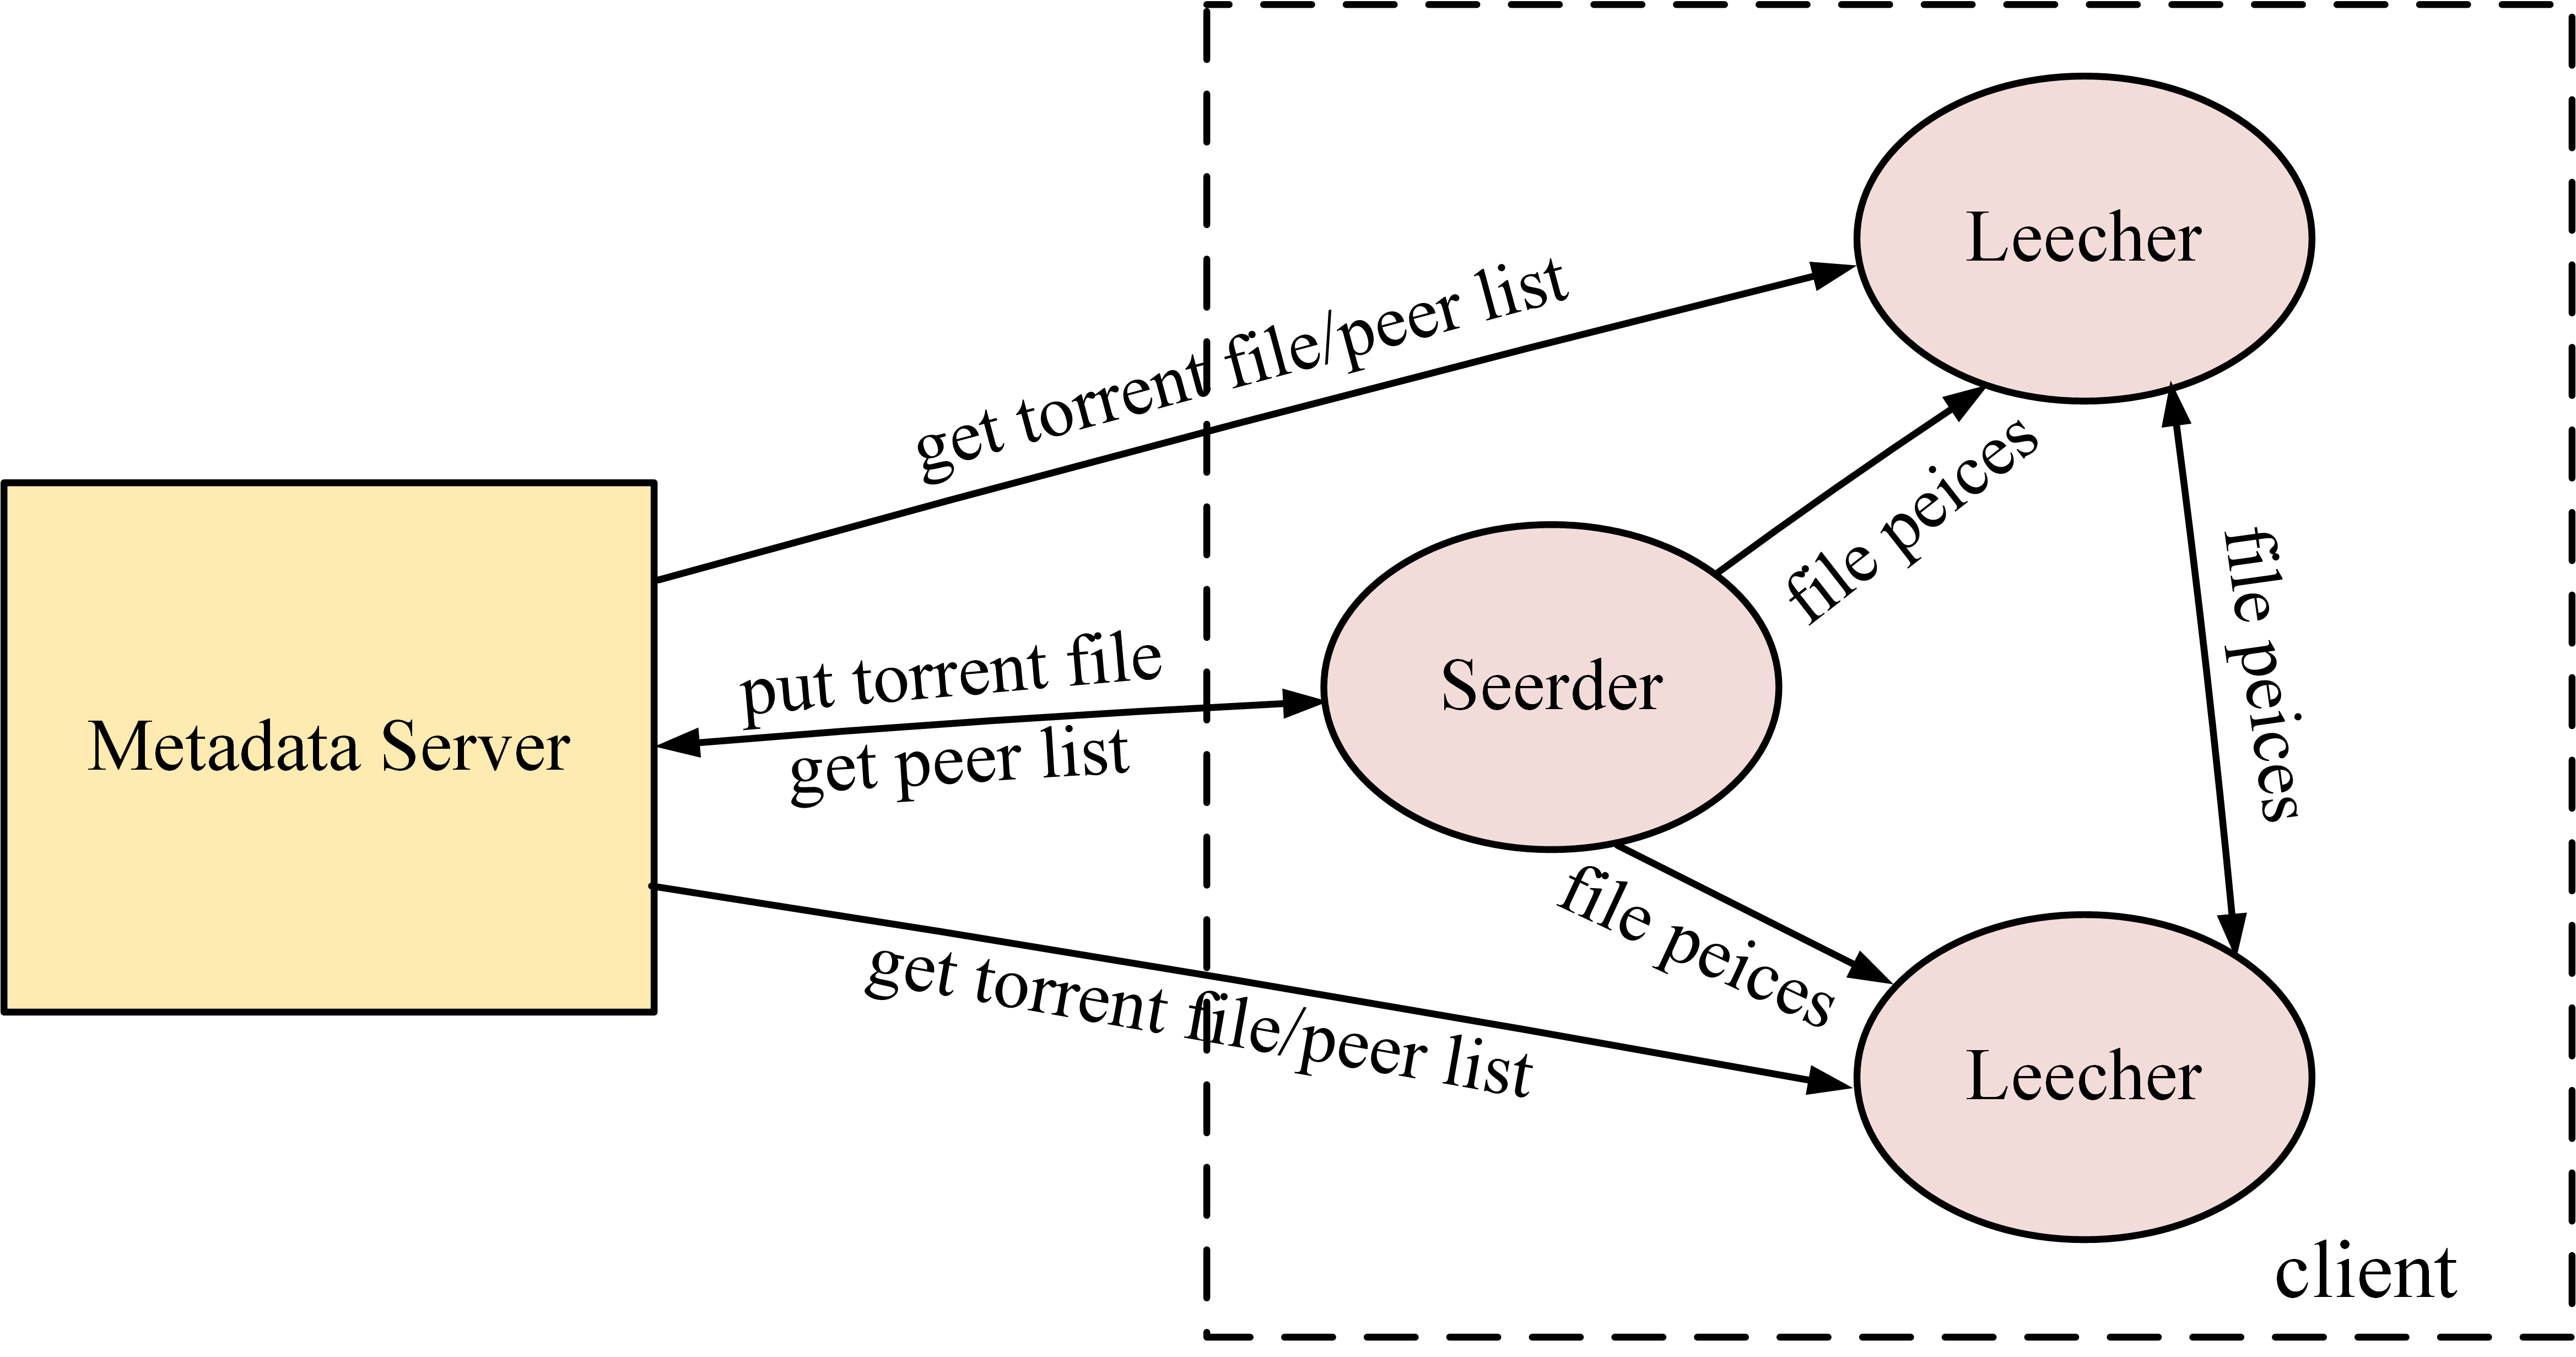
\includegraphics[width=2.9in]{f3.png}
		\caption{System Architecture}
		\label{fig:side:1}
	\end{figure}
	
	In our design, we use Apache ZooKeeper to act as a metadata server which provides the information of peer lists of each swarm and metainfo of each file. The top level directories in ZooKeeper consist of /peer and /file nodes. The /peer node is used to hold the hostname and port number information of each peer. The /file nodes maintains the files and swarms.  Each file is associated with a descendant node under /file, we store the  torrent content in the file node's data. All peers within one file swarm are registered under that specific file node.
	
	A client can be started either as a seeder or as a leecher with a unique peer ID. If the user has a file to share, he can start the client as a seeder. The client will create a metafile and advertise the file to the ZooKeeper. A node with filename as node's name is created under /file and the contents of the torrent information include filename, file size,  piece length, pieces will be stored in the node. Meanwhile, the peer is registered under both the /peer node and /file/filename node with the peer ID as the node's name and hostname and port number as the node's data. If the user wants to download a file, he needs to initiate the client as a leecher with the file's name. The client will retrieve the metafile and peer lists associated with the file from the ZooKeeper. The peer is also added to the lists. Then the client can connect to those peers in the returning list to start exchange file pieces. Downloading or uploading multiple files simply involves running multiple client instances.
	
	\subsection{Connection state}
	A peer must maintain state information for each connection that it has with a remote peer. A peer usually play the roles of both downloader and uploader, Figure 2 shows two finite state machine for these two actions.
	
	\begin{figure}
		\centering
				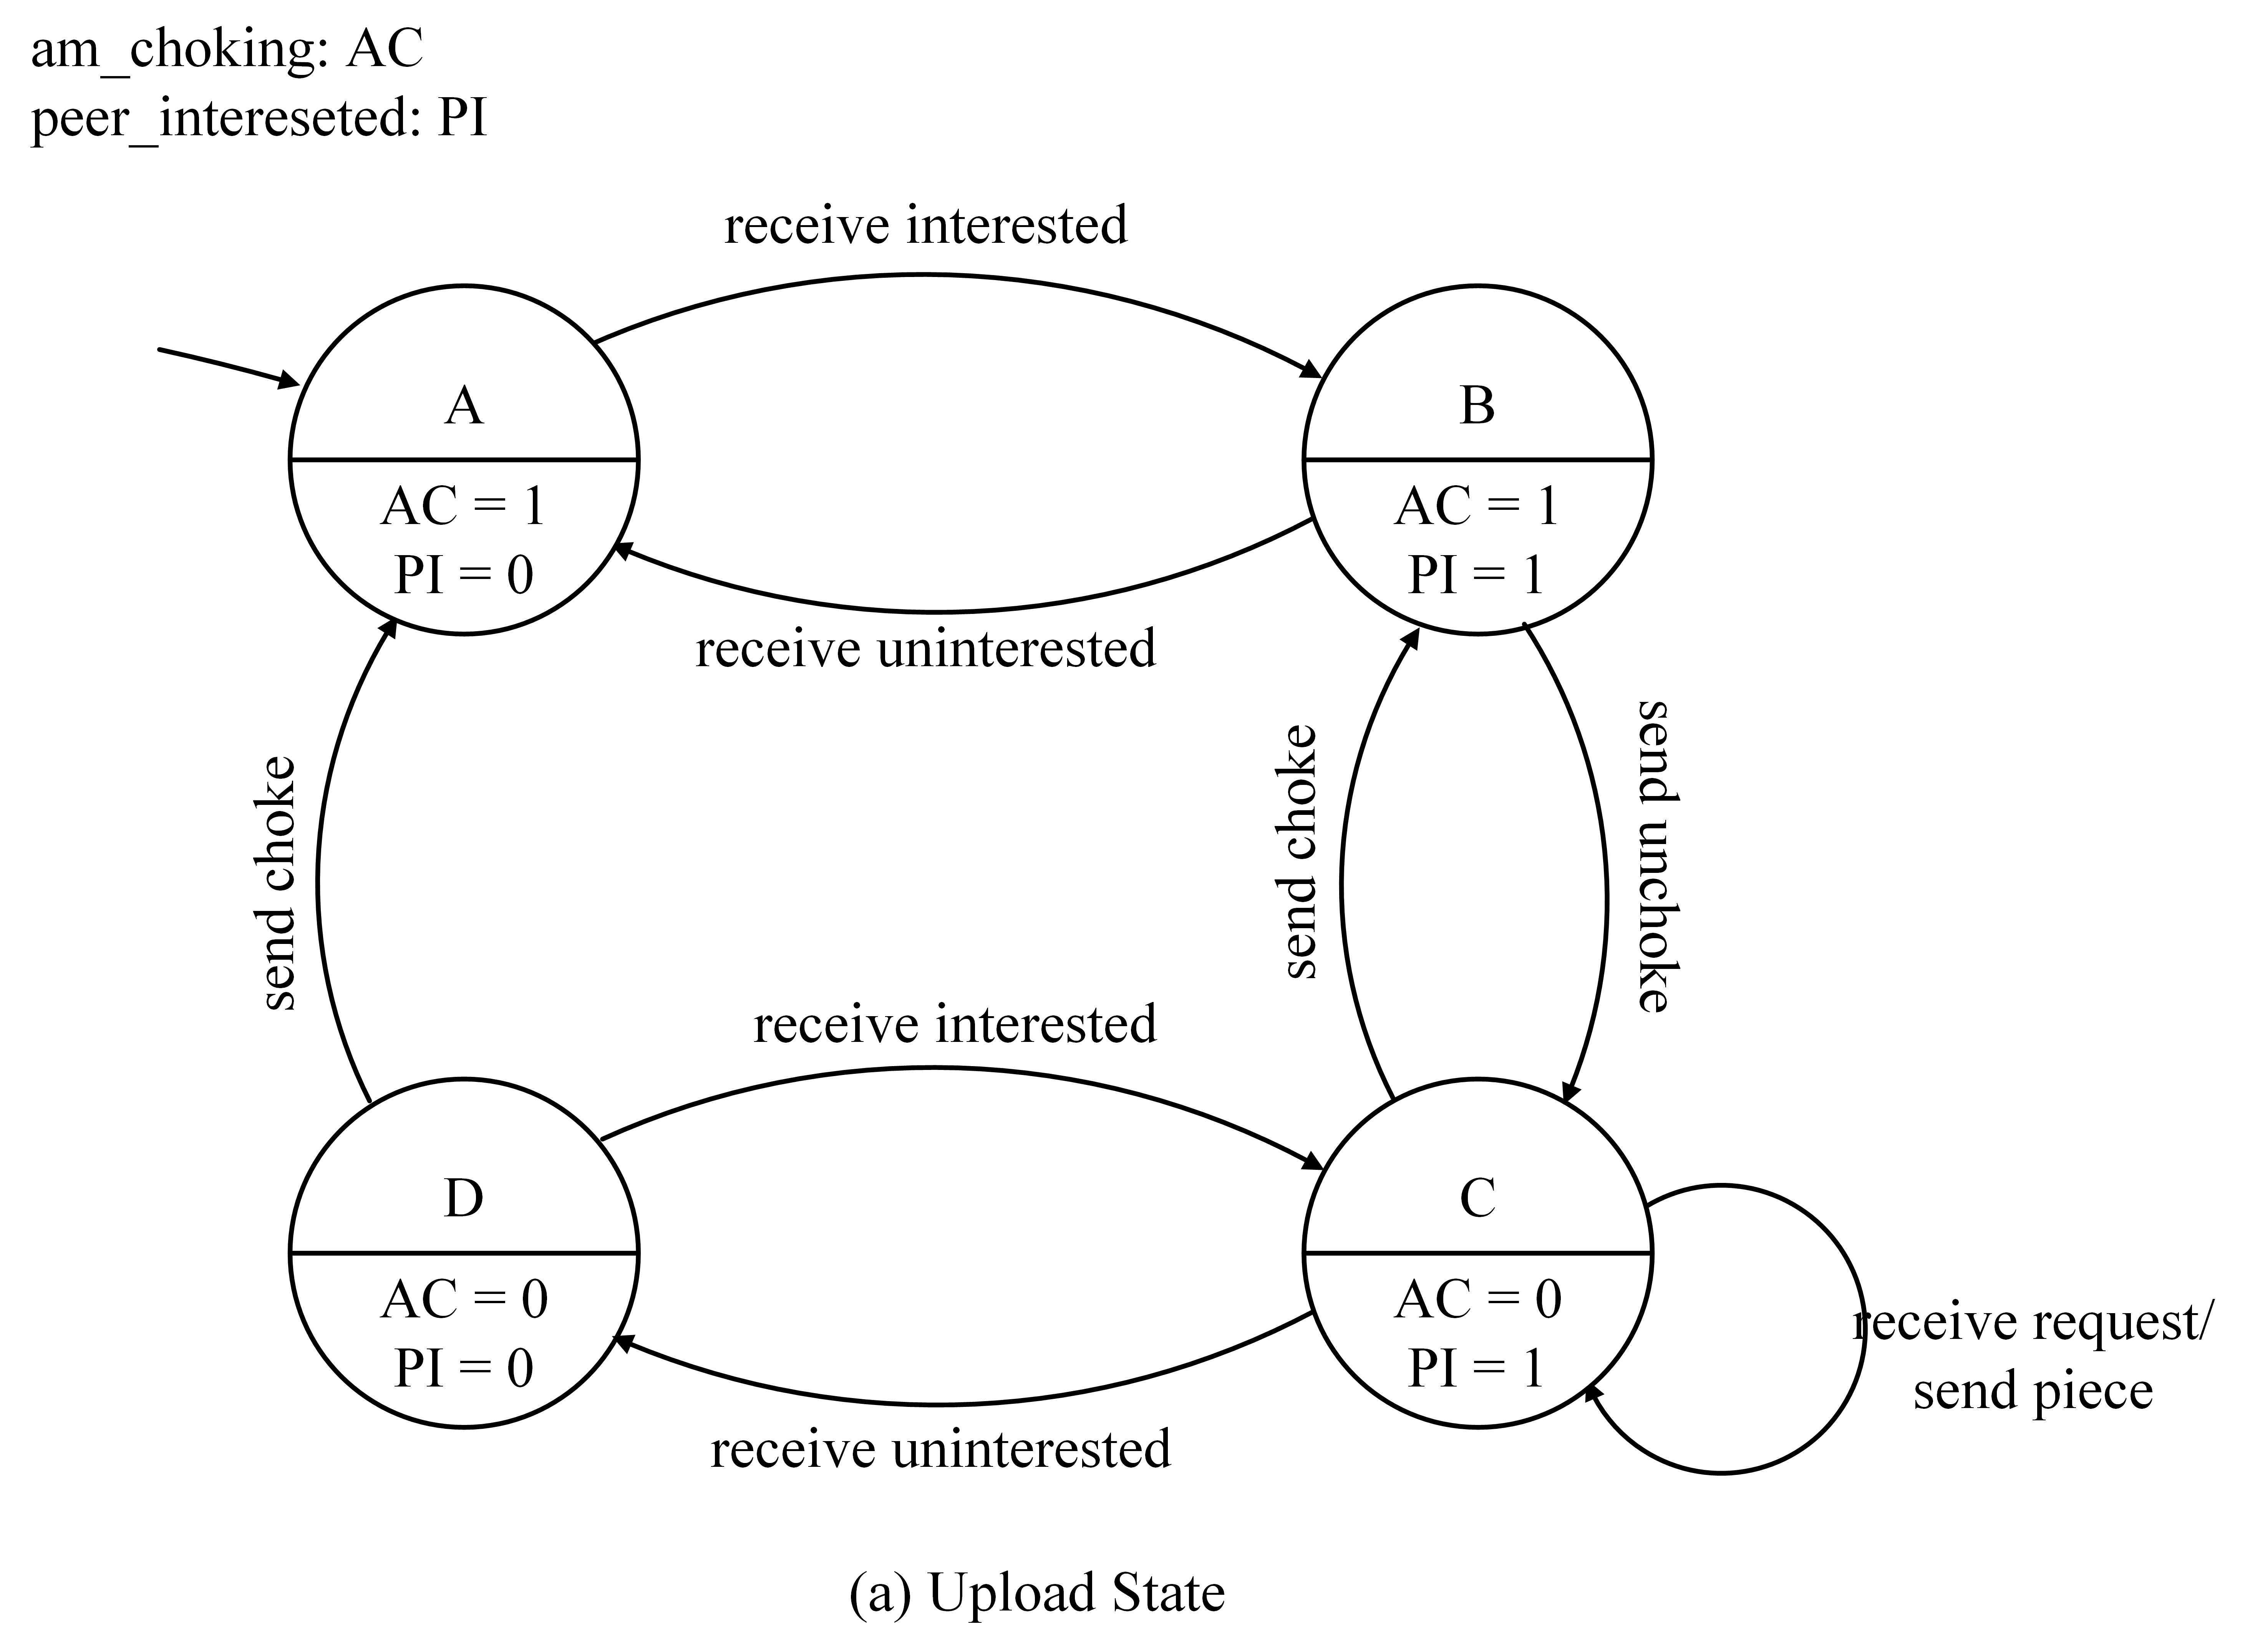
\includegraphics[width=0.9\linewidth]{f1.png}
				\label{fig:sub1}
			
				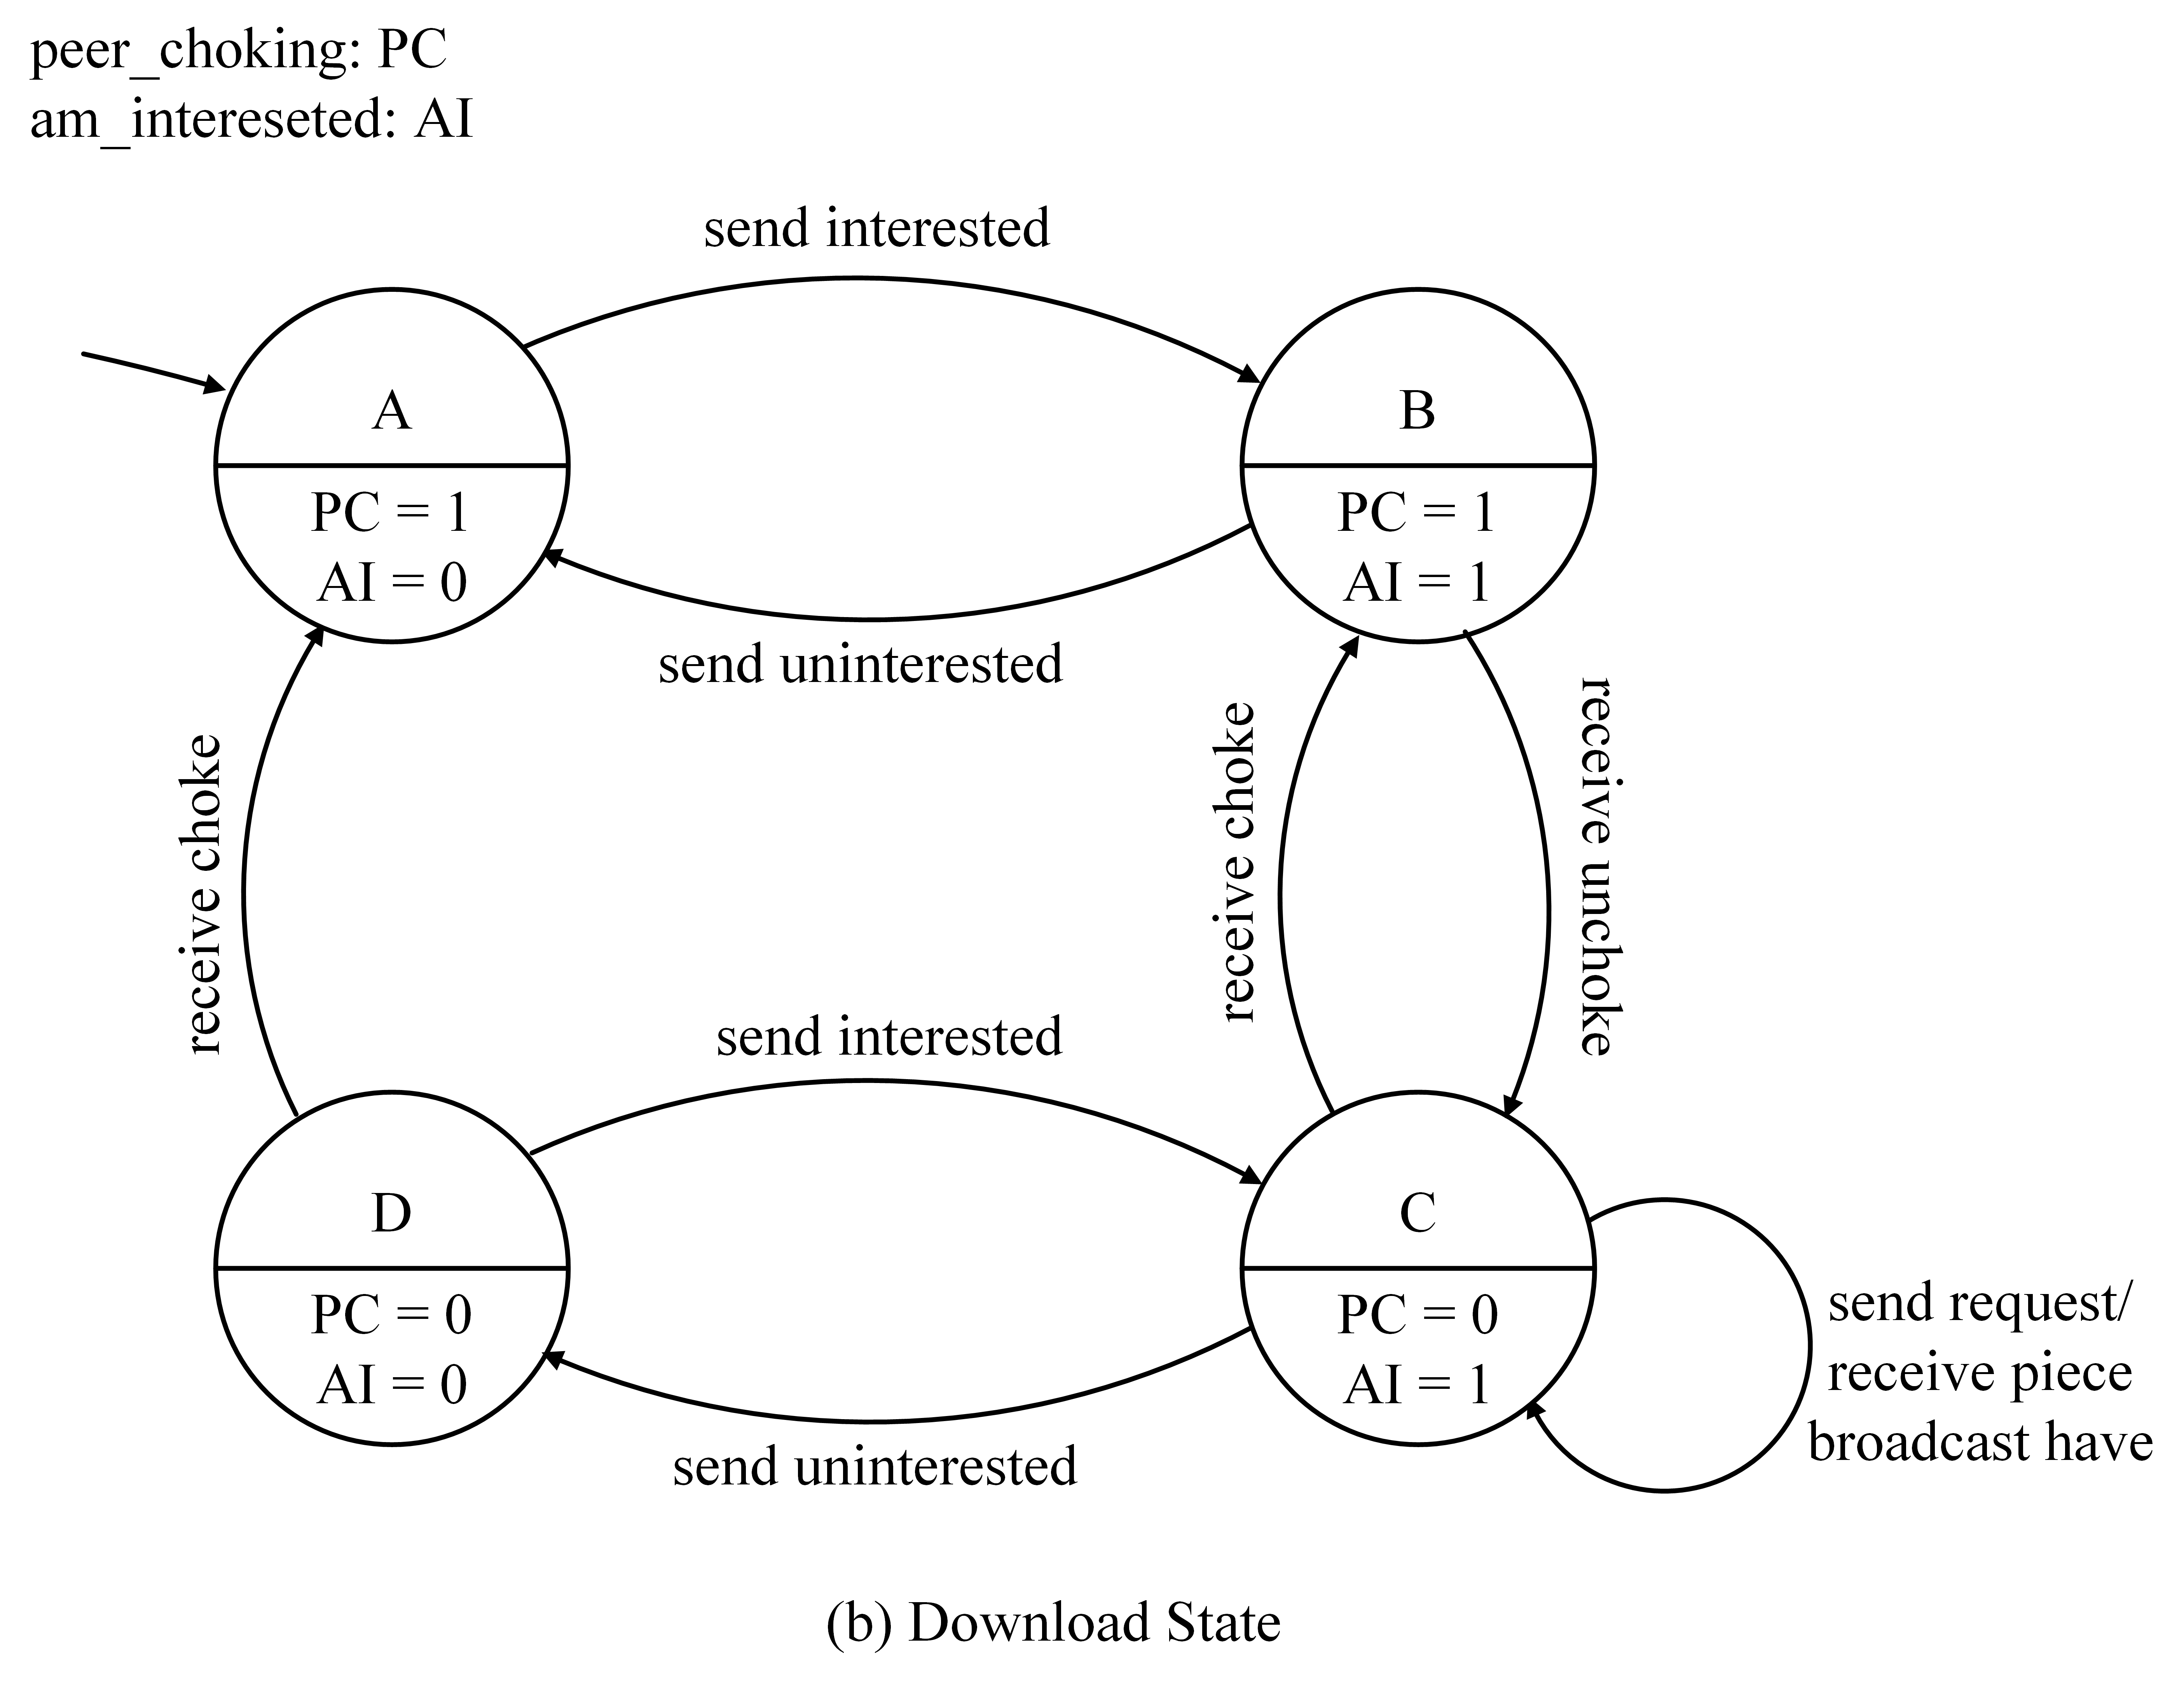
\includegraphics[width=0.9\linewidth]{f2.png}
				\label{fig:sub1}
		\caption{Connection State}
		\label{fig:side:b}
	\end{figure}
	

	
	\subsection{Deal with churn}
	The dynamics of peer participation, or churn, are an inherent property of Peer-to-Peer  systems and critical for design. In our system, each client spawns a listening thread to accept new connections from peers joining the swarm later. If receive handshake message successfully, current peer will add the new peer into its peer list. To deal with dropping offline peers, as every node is registered in the metadata server, we set a watch for each peer to monitor the file's node they involve in. If any node in the swarm changes, the peer will be informed and pull the updated peer list from the metadata server with dead peers removed.
	
	\subsection{Choking mechanism}
	Each peer always unchokes a fixed number of other peers which allows TCP's built-in congestion control to reliably saturate upload capacity\cite{BitTorrent}. This is decided periodically. In our implementation, a scheduled task is executed at a fixed rate to decide the unchoked sets. For simplifying, we calculate the download rates of all other peers that the current peer provide uploadings to, picks \emph{k} peers who has the fastest rate. If a peer in the unchoked set is choked previously, then the current peer will send unchoke message to that peer.
	
	\subsection{Piece selection}
	Selecting pieces to download in a good order is very important for transfer efficiency. For example, if all the peers start to download the first piece from the first bit of the bitfield, it results in all peers having same bits of pieces, and can not exchange files with each other. In our design, we adopted the random first piece algorithm. The peer will check its own bitfield, pick the bit with zero randomly and request that index of piece from other peer.
	
	\subsection{File integrity check}
	The data of /filename znode has a string called pieces, in which 20-byte hash values related to each piece of the file respectively are concatenated. Secure Hash Algorithm 1(SHA1) produces a hash value for each piece and render it as a hexadecimal number. These SHA1 values, regarded as message digests, give us a favor to check if the file is completely downloaded during carrying on experiments. 
	
	\section{Experiments and results}
	Our system is tested on ecelinux[1-3].uwaterloo.ca. The ZooKeeper service is on snorkel.uwaterloo.ca. The measurements focus on fault tolerance and evaluation of performance. We ran the system with three sizes-small, medium, large- of files of various types. There are 6 peers in this experiment, one is the seeder and the other 5 are leechers. In each test, a peer as seeder is started at the beginning, then different numbers of leechers ran simultaneously or non-simultaneously. 
	
	\subsection{Fault tolerance}
	For fault tolerance, as the centralized tracker is already eliminated in our design, ZooKeeper introduce failures to peers. There are two kinds of potential failures: uploader failure and downloader failure.
	
	After killing several uploaders, existing alive peers get an updated peer list. They close the connection with those “died” peers and then keep contact with peers still on the list along with exchanging file pieces. 
	
	On the other hand, we killed a particular peer who acts as a downloader before finishing and then restarted it to find out if it has capability to recover unfinished download task.
	When peers finish downloading, we examined the downloaded file by comparing its hash value generated by Secure Hash Algorithm 1(SHA-1) with that of the original file to check the correctness.
	
	The experimental results prove that our implementation is able to handle both situations well.

	
	
	
	
	\subsection{Evaluation of  performance}
	Performance refers to the transfer rate and download duration in terms of ranging swarm size and file size. files are split into fixed-size pieces which are all the same length of 256K except for possibly the last one which may be truncated. Unchoke interval for the choke task is 1s, unchoke slot is set to contain 4 peers. All the tests are run 10 times and all results are averages from 10 runs. 
	
	\subsubsection{Performance as a Function of the Swarm Size(number of seeders)}
	This experiment aims to show that BitTorrent performance improves with increasing seeder size. The data points are collected through running experiments with swarm sizes 1 to 5. At each run, one new peer joined a swarm until completing download. The swarm was initially created with one seeder then the rest 5 peers entered the swarm one by one after the preivous peer finishing downloading. Thus, peers that obtain the complete file can be seen as seeders. That is ``n seeders-one leecher''. 
	
	Table 1 shows the measured download time of newly joined peer of 10 runs for the tests. The file size is medium. Figure 3 and 4 represent average download time and average download rates for newly-joined peers. The performance increases as seeder size changed from 1 to 5. 
	
	
\begin{table}
	\caption{Download Time of Different Seeder Sizes}
	\begin{center}
		\begin{tabular}{cccccc}
			\hline
			\rule{0pt}{12pt}Test \#  & \rule{0pt}{12pt}size 1   &\rule{0pt}{12pt} size 2  &\rule{0pt}{12pt} size 3 &\rule{0pt}{12pt} size 4 &\rule{0pt}{12pt} size 5\\
			\hline\rule{0pt}{12pt}
			1    &   17874 & \ 	12086 & \ 	6817 & \ 	6802 & \ 	7904 \\
			2    &   14305 & \ 	11394 & \ 	5278 & \ 	7288& \ 	6897 \\
			3    &   19312 & \ 	9793 & \ 	9747 & \ 	7229& \ 	7901 \\
			4    &   25102 & \ 	9825 & \ 	8751  & \ 	8734& \ 	6208\\
			5    &   23135 & \ 	10915 & \ 	11600 & \ 	6765 & \ 	5856\\
			6    &   24998 & \ 	12018 & \ 	7847 & \ 	7138 & \ 	6299\\
			7    &   20161 & \ 	9402 & \ 	6862 & \ 	8708 & \ 	6102\\
			8    &   25185 & \ 	15401 & \ 	9814 & \ 	7876 & \ 	7778\\
			9    &   24632 & \ 	10248 & \ 	10264 & \ 	7834 & \ 	7323\\
			10    &   21093 & \ 	12885 & \ 	8194 & \ 	6737 & \ 	6789\\
			\hline\rule{0pt}{12pt}
			Average(ms)    &   21579.7 & \ 	11396.7 & \ 	8517.4& \ 	7511.1  & \ 	6905.7 \\
			\hline
		\end{tabular}
	\end{center}
\end{table}

\begin{figure}
	\centering
		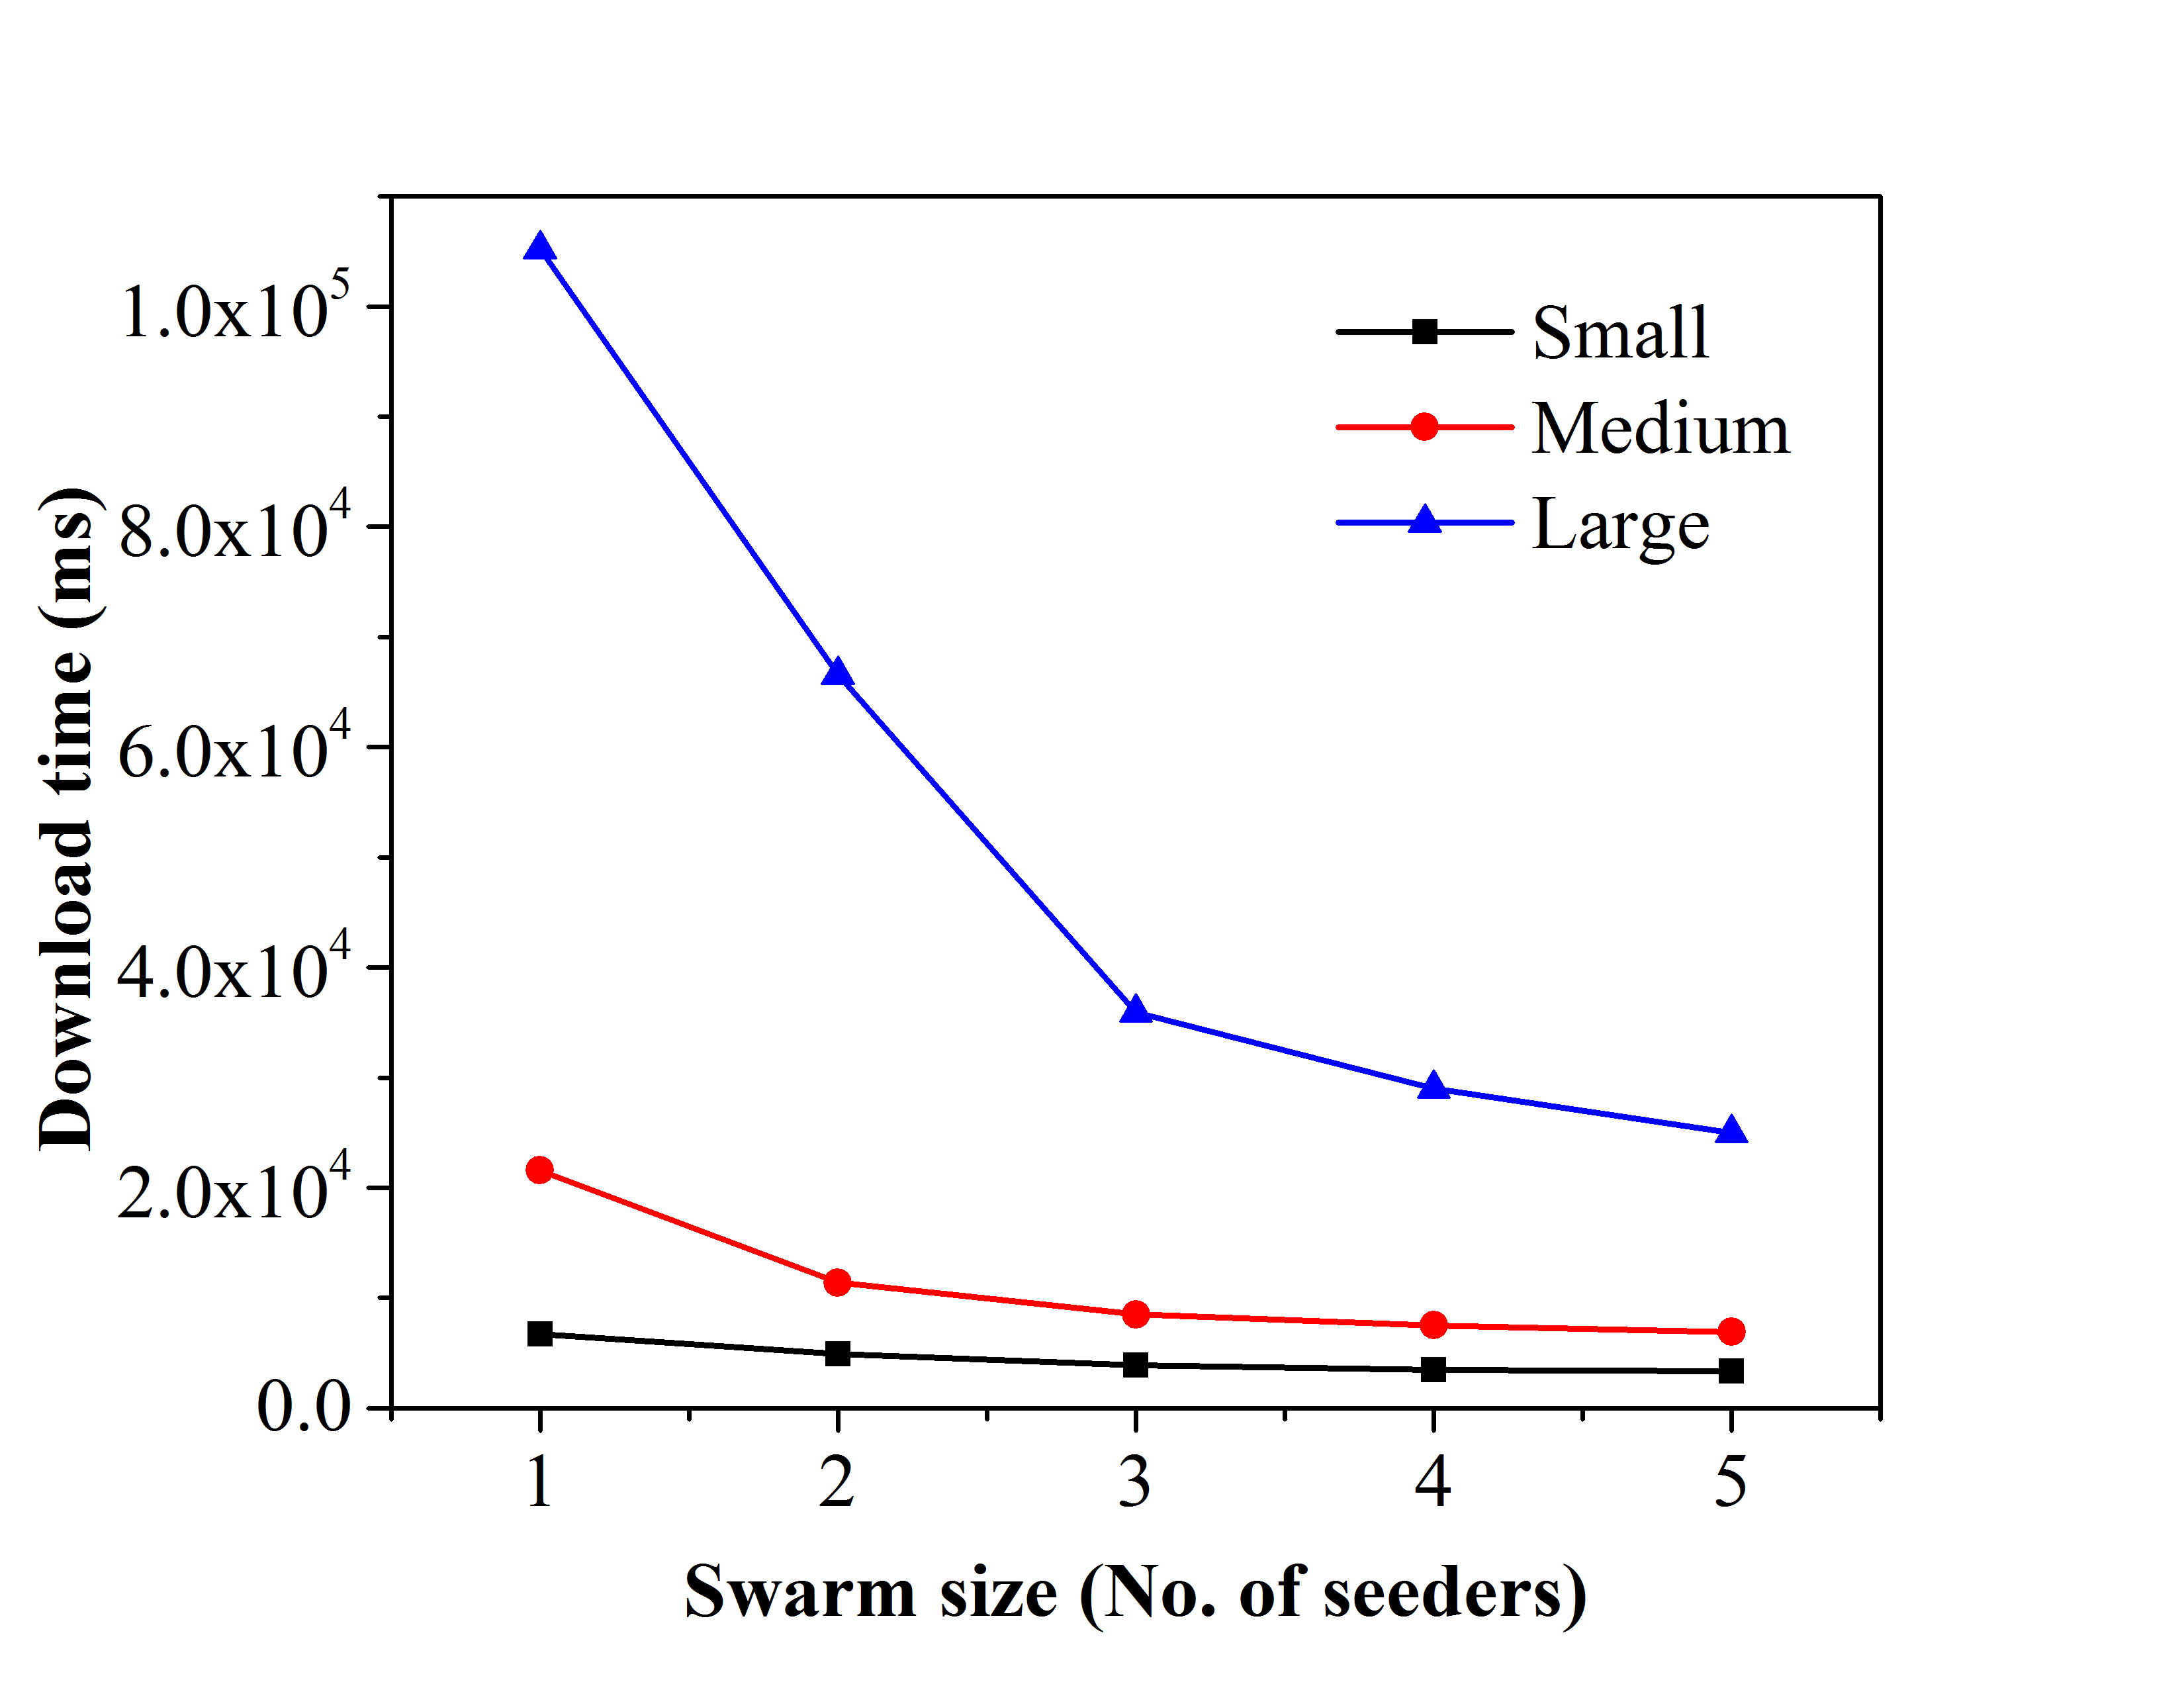
\includegraphics[width=2.8in]{Graph1.png}
		\caption{Download Time vs. Seeder size}
		\label{fig:side:a}
\end{figure}

\begin{figure}
	\centering
	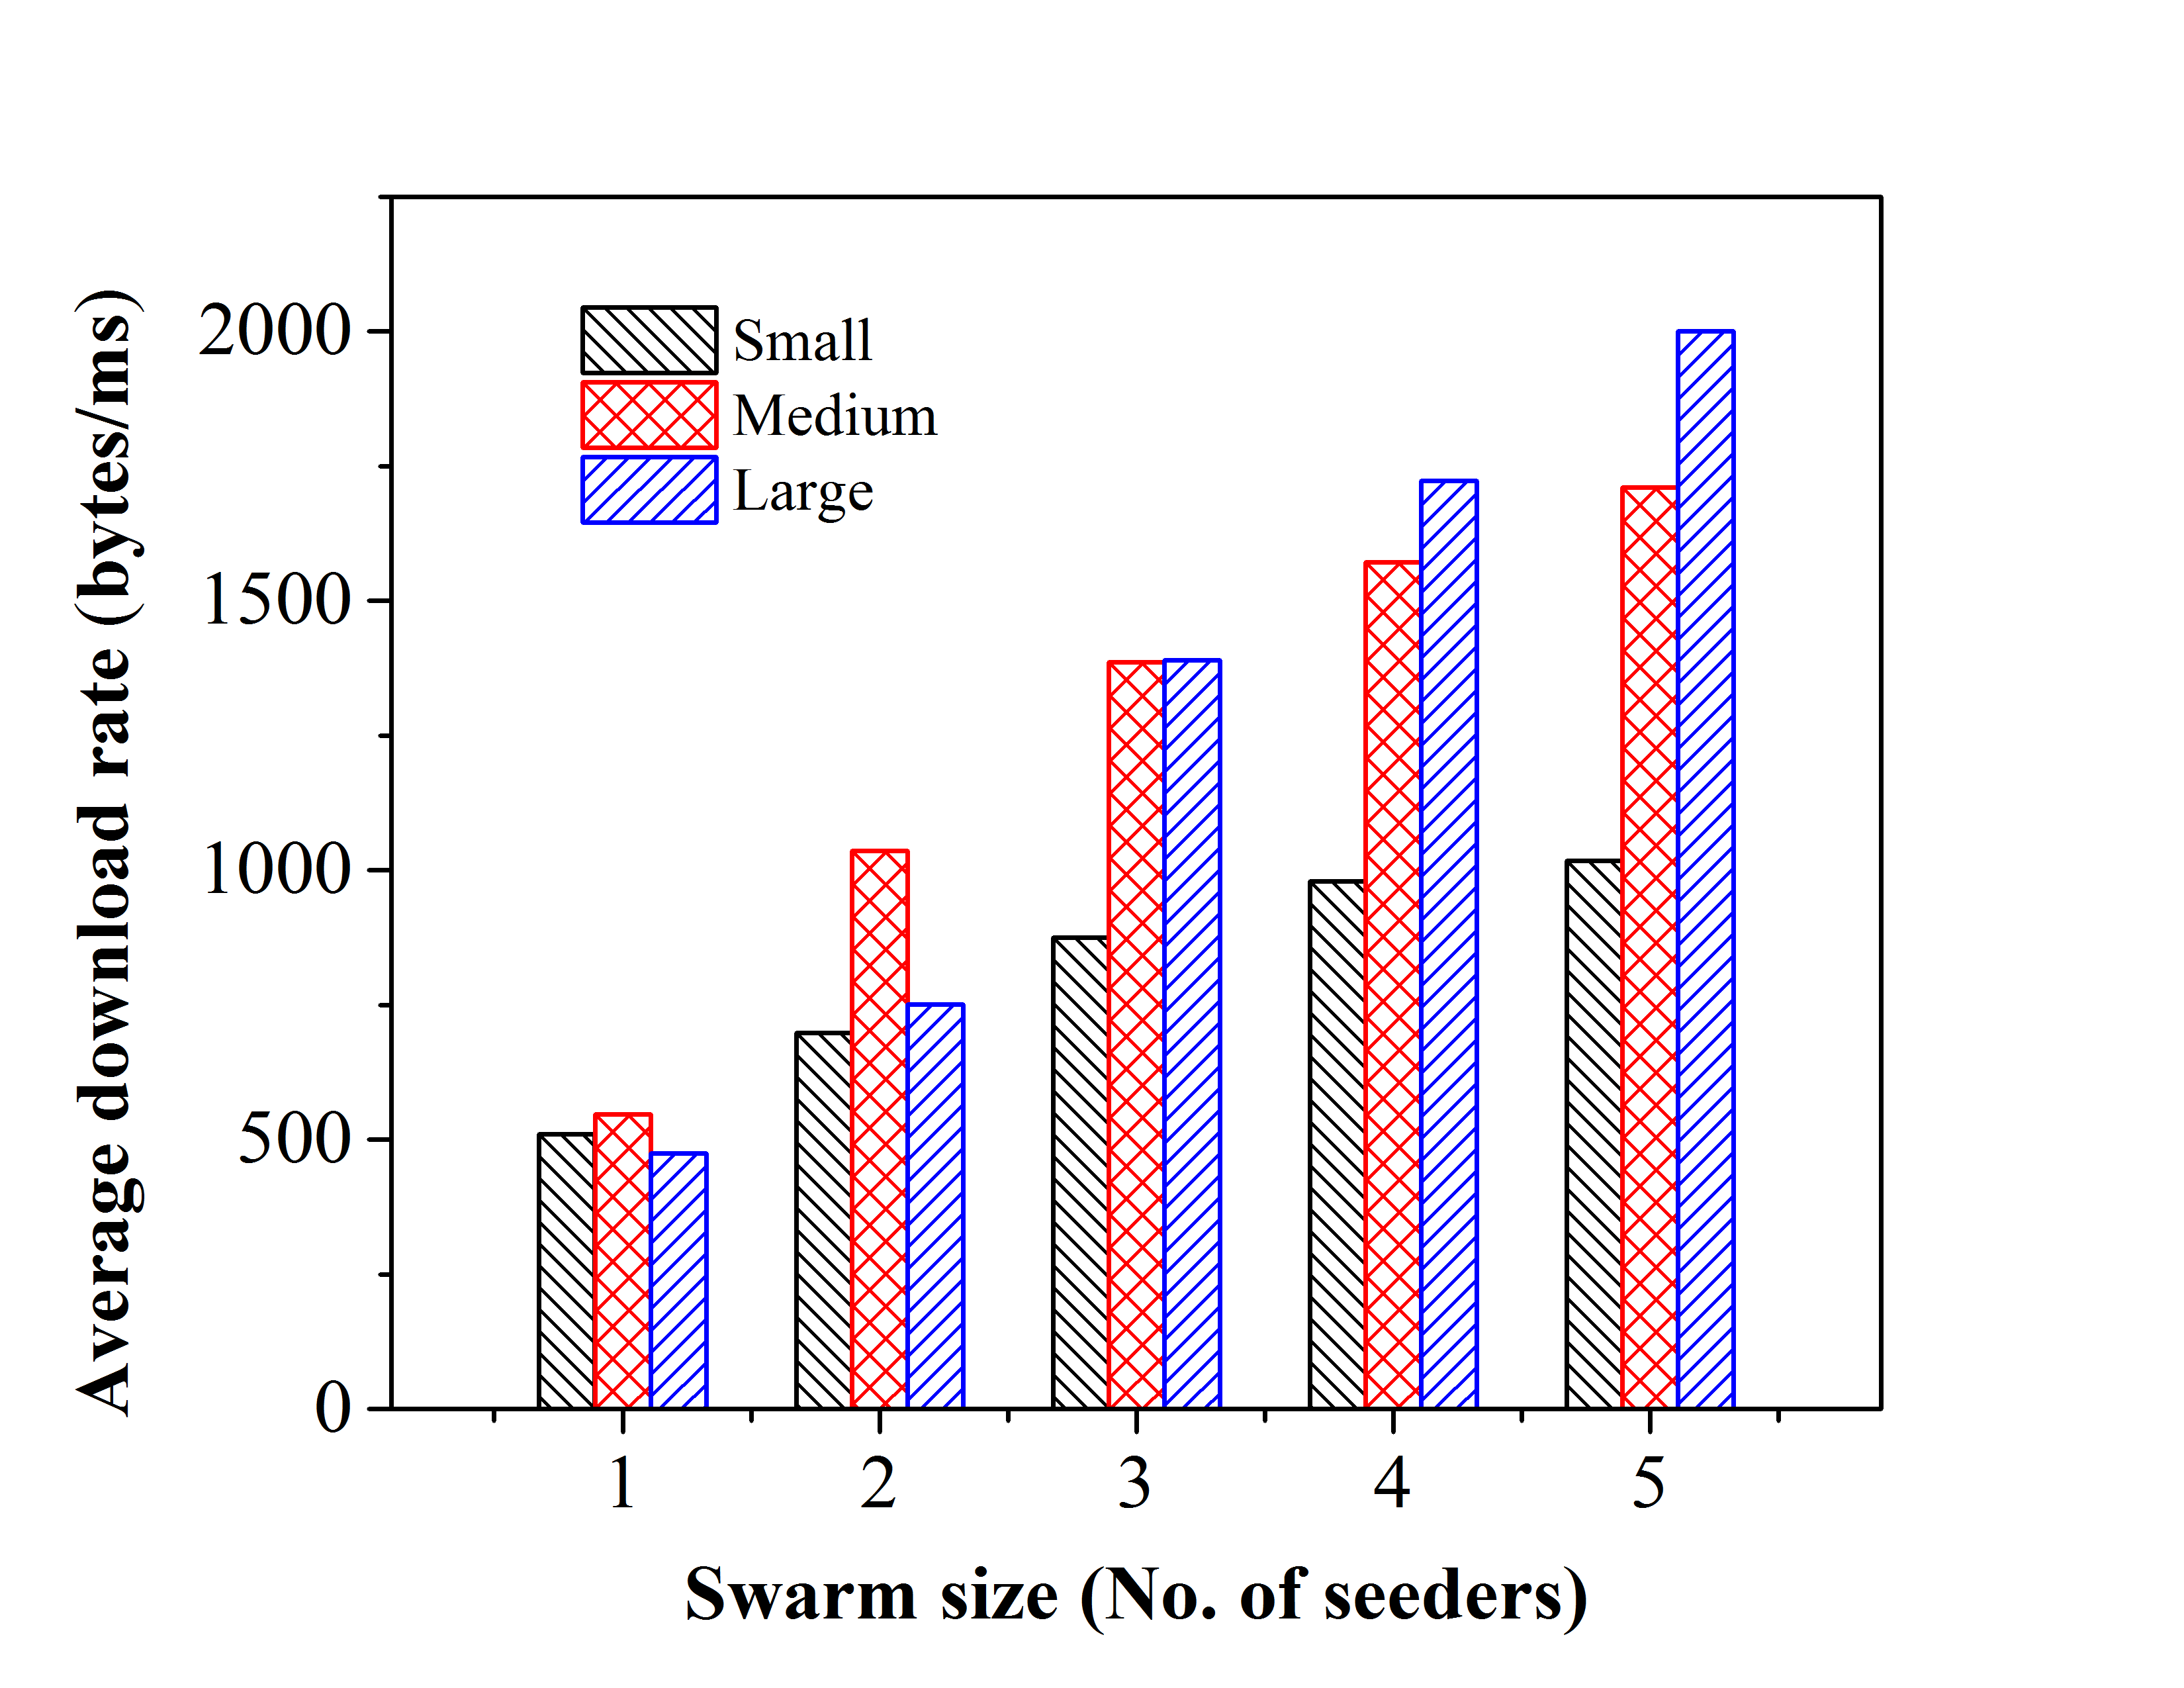
\includegraphics[width=2.8in]{Graph2.png}
	\caption{Average Download Rate vs. Seeder size}
	\label{fig:side:a}
\end{figure}

	The results show that larger swarm performs better than smaller one. We see that the the performance of average download time and download rate for all 3 sizes files increases as the swarm size increases. It is obvious that the larger sizes the swarms are, the more peers that can provide file pieces to the new peer so that the download can speed up. We also notice that the decrease of download time is dramatical form size 1 to size 3 and then tends to flat. One possible reason for this tendency is that with more providers, the leecher may send redundant requests and messages which affects the efficiency.	
	
	\subsubsection{Performance as a Function of the Leecher Size(number of leechers)}
	In this experiment, the swarm is initiated with one seeder and then we start different number of leecher peers in the same time making their download simultaneous. This is ``one seeder-n leecher''. The measurement of performance is for 1, 3, and 5 newly-joined leechers respectively. The download time and average transfer rate is shown in table 2-5.
		\begin{table}
			\caption{Average Download Time of 1 Leecher}
			\begin{center}
				\begin{tabular}{ccc}
					\hline
					\rule{0pt}{12pt}file size  & \rule{0pt}{12pt}medium(ms) & \rule{0pt}{12pt}large(ms)\\
					\hline\rule{0pt}{12pt}
					 leecher\_1   &    21579.7 
					    & \   105223.1  \\
					\hline
				\end{tabular}
			\end{center}
		\end{table}
		
	\begin{table}
		\caption{Average Download Time of 3 Leechers}
		\begin{center}
			\begin{tabular}{ccc}
				\hline
				\rule{0pt}{12pt}file size  & \rule{0pt}{12pt}medium(ms) & \rule{0pt}{12pt}large(ms)\\
				\hline\rule{0pt}{12pt}
				leecher\_1   &    10291.7 & \   35817.2   \\
				leecher\_2   &    1066.5 & \   34736.4 \\
				leecher\_3   &    10467.5& \  33409.6  \\
				\hline\rule{0pt}{12pt}
				Average   &   10275.2 & \  34654.4   \\				
				\hline
			\end{tabular}
		\end{center}
	\end{table}
	
		\begin{table}
			\caption{Average Download Time of 5 Leechers}
			\begin{center}
				\begin{tabular}{cccccc|c}
					\hline
					\rule{0pt}{12pt}file size  & \rule{0pt}{12pt}medium(ms) & \rule{0pt}{12pt}large(ms)\\
					\hline\rule{0pt}{12pt}
					leecher\_1   &    9348.7 & \   28307.3    \\
					leecher\_2   &    10477.0 & \   27830.9 \\
					leecher\_3   &    10561.6& \  	26701.2  \\
					leecher\_4   &    9757.1 & \   26273.5  \\
					leecher\_5   &    9252.& \ 27462.6  \\
					\hline\rule{0pt}{12pt}
					Average   &    9879.4  & \  27315.1  \\	
					\hline
				\end{tabular}
			\end{center}
		\end{table}
	
		\begin{table}
			\caption{Average Download Rate of Different Leecher Sizes}
			\begin{center}
				\begin{tabular}{cccc}
					\hline
					\rule{0pt}{12pt}file size  & \rule{0pt}{12pt}size\_1   &\rule{0pt}{12pt} size\_3  &\rule{0pt}{12pt}size\_5\\
					\hline\rule{0pt}{12pt}
					medium(byte/ms)   &    547.17 & \ 	1149.1 & \ 	1195.2 \\
					large(byte/ms)    &   474.68 & \ 	1441.3 & \ 	1828.6  \\
					\hline
				\end{tabular}
			\end{center}
		\end{table}
	
	Comparing the results in these tables, we see that the average download time of every leecher peer decreases as the leecher number increases and the average rate
	increase accordingly. All leechers are started concurrently and they are downloading the same file, the improvement of their performance is due to the advantages of Bittorrent protocol that peers can share pieces with each other during downloading. Another reason is that we adopted the random piece selection algorithm so that the peers are very likely to obtain different pieces at the very beginning, thus they can upload to and download from others simultaneously. This balances the load from the only seeder to all peers.
	
	\subsubsection{Estimated Instantaneous Rate}
	The estimated instantaneous rate here is defined as a ``windowing" average rate which is the bytes length per piece received divided by the time difference between current piece received and last piece received. We plot the instantaneous rate with time from the download established to download finish in Figure 5. We fitted the curve with polynomial fitting. 
	
	We can see that instantaneous rate slows down after about 81\% completion. There are two reasons for this tendency. One is that the peer select piece it does not own randomly. In our implementation, we generate a random index number and check this index with local peer's bitfield to decide whether the peer need to request. Thus, when most of the bitfield is already set, it requires more runs to generate an index of bitfield which is not set yet. The other reason is that the peer may send multiple requests for same piece to remote peers and receive redundant content. To speed this up, the peer can send requests for all of its missing pieces to all remote peers and enable cancellation every time a piece arrives.
	
	\begin{figure}
		\centering
		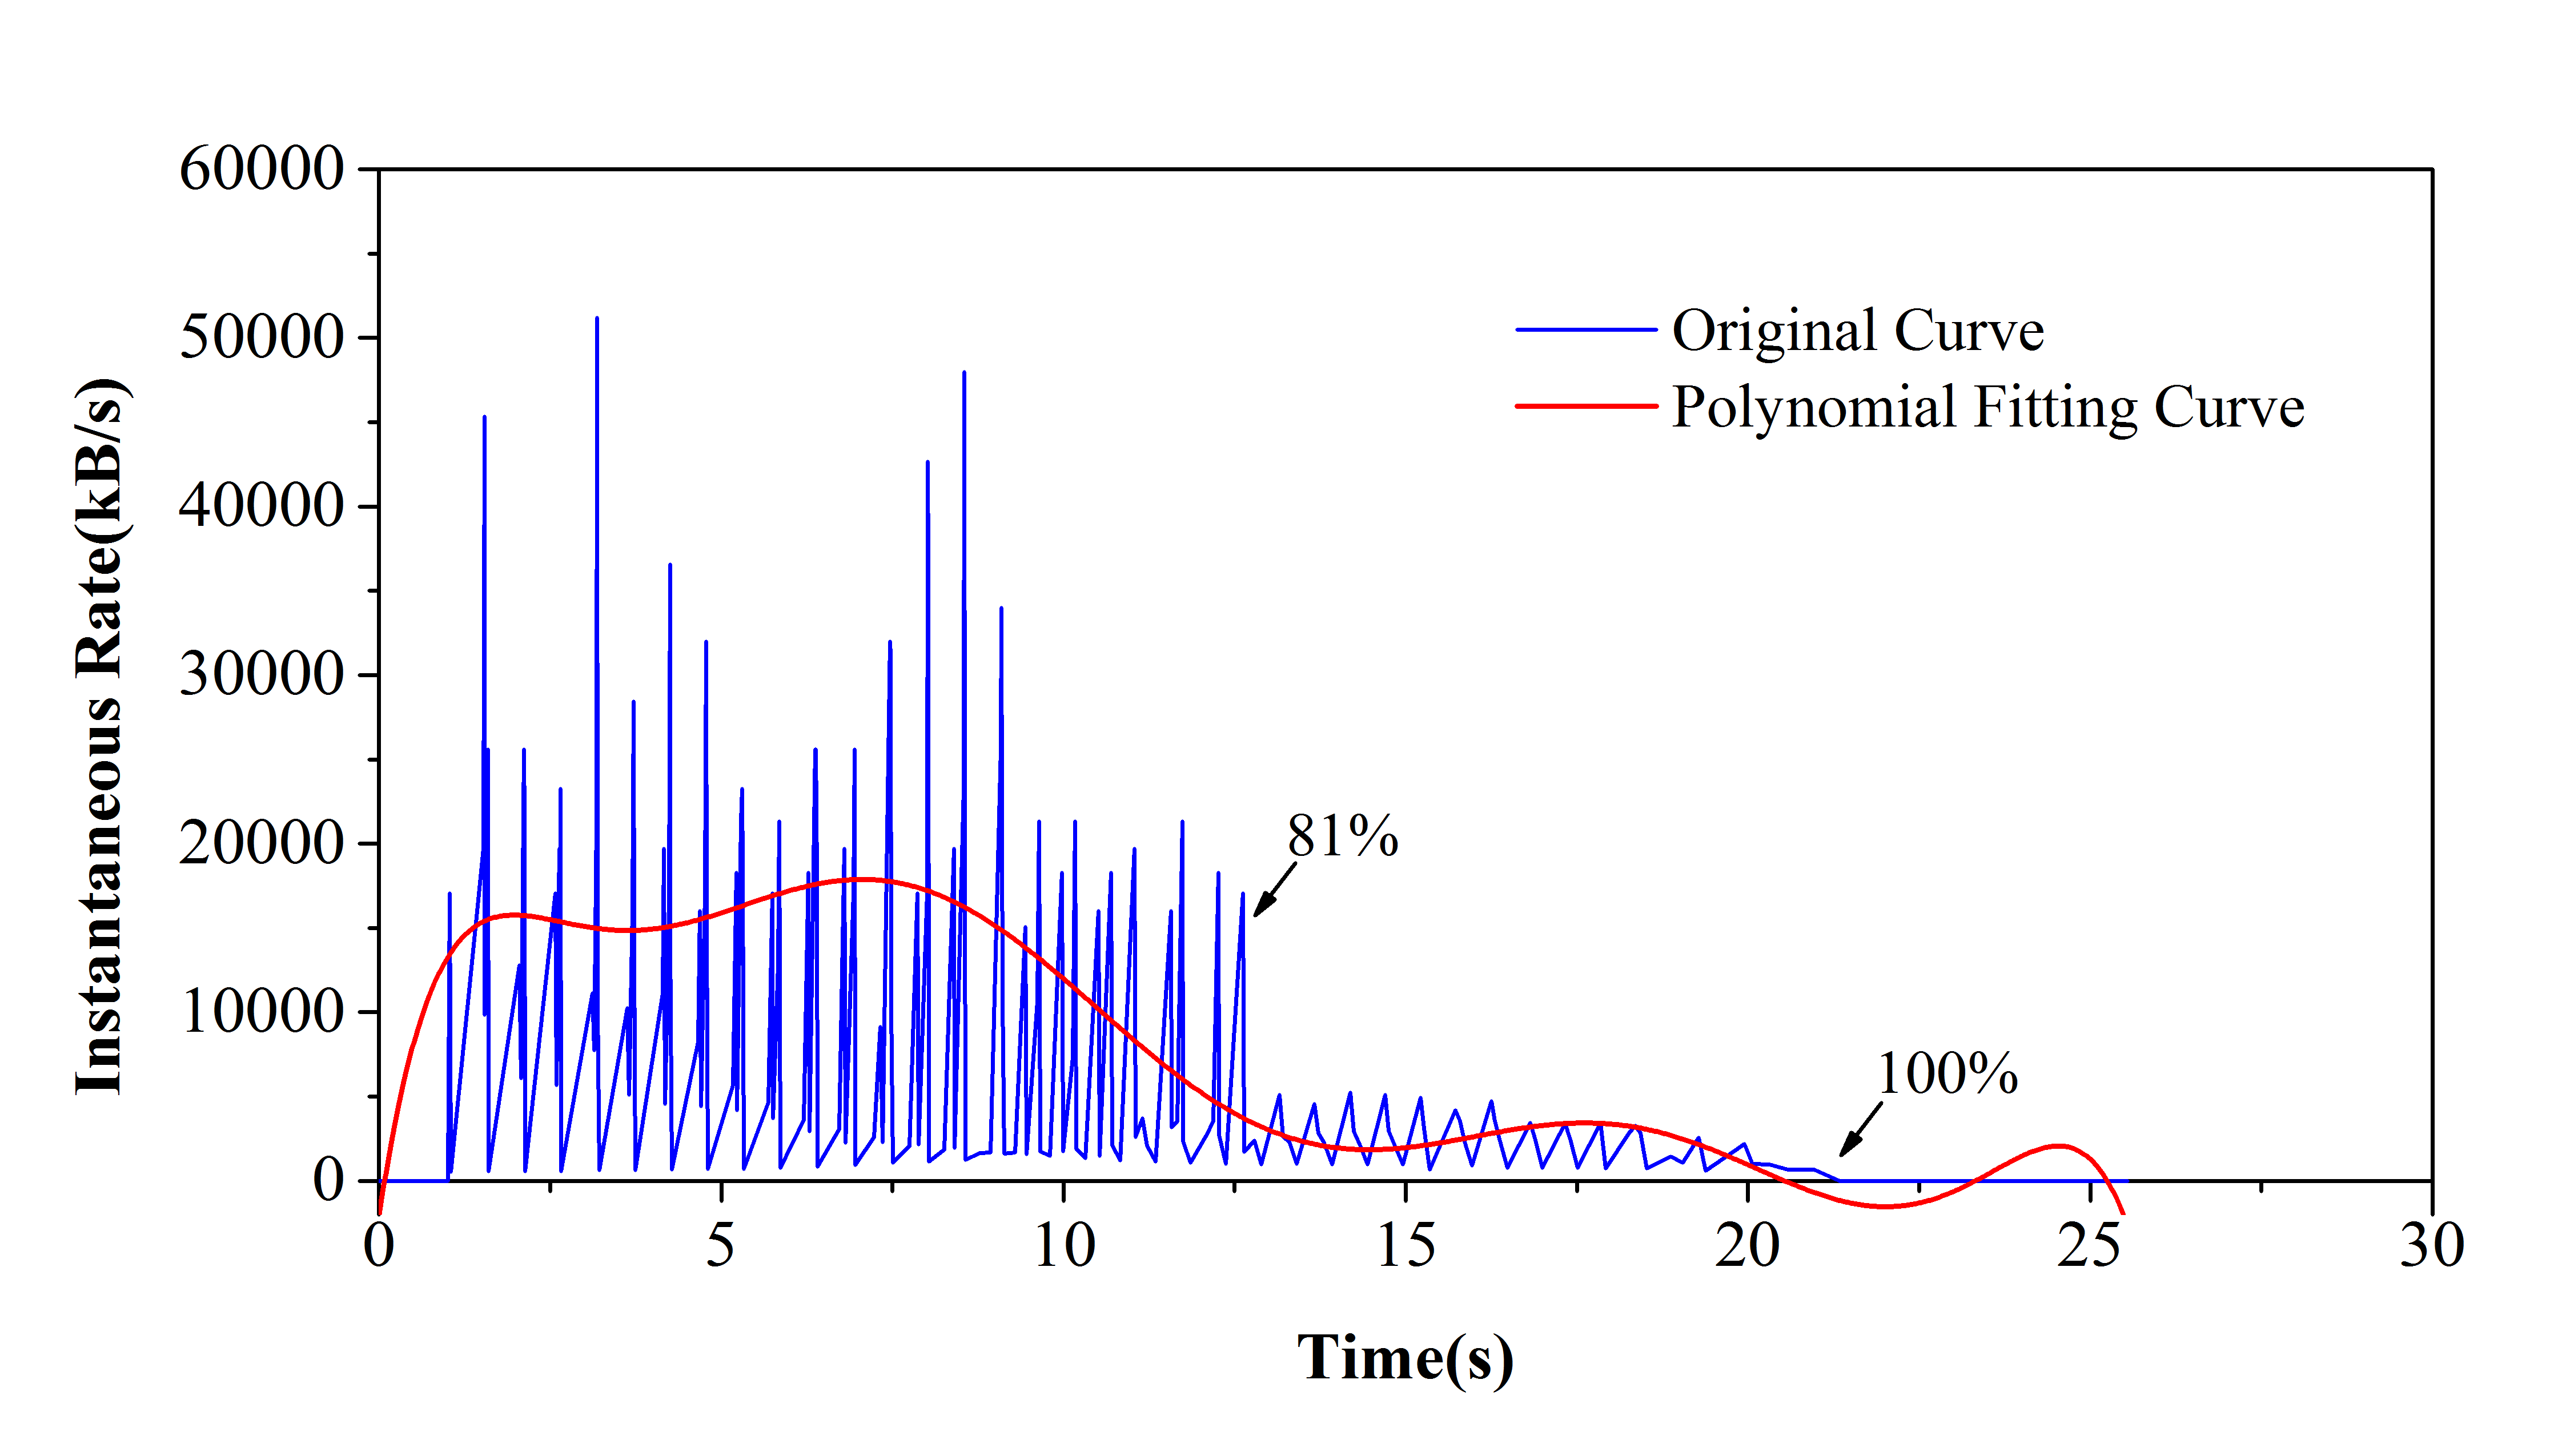
\includegraphics[width=0.5\textwidth]{Graph5.png}
		\caption{Estimated Instantaneous Rate vs. Time}
		\label{fig:side:f}
	\end{figure}
	
	
	\section{Conclusion and future work}
	This paper reveals a BitTorrent-like system, which is a decentralized peer-to-peer file sharing system. This work uses ZooKeeper to replace the metainfo file(.torrent) and tracker in native BitTorrent protocol, thus improving bootstrap and reducing messages flowed in the network.
	
	A new observation of free-riding problem in BitTorrent has experimentally demonstrated\cite{free-riding in BitTorrent} by Sirivianos and Chen regardless of tit-for tat mechanism. When a peer connects to many peers, it increases its chance to be unchoked by leechers and find out seeders. As a result, it may adopt an exploit strategy. Some modifications should be made in the system to allow peers to detect whether a peer tries to become selfish or not before establishing a connection with it.
	
	For the reason that tit-for-tat strategy upload speed to determine which peers will be put in unchoked list, those new entrants without any data have no opportunity to start downloading before some peers finish. Consequently, we will add a new mechanism that enables new peers to upload a piece randomly when they take part in the network. Moreover, an extra unchoked space is offered to give those new peers or peers with a low download/upload rate a chance.

	% conference papers do not normally have an appendix
	
	
	% use section* for acknowledgment
	%\section*{Acknowledgment}
	
	
	%The authors would like to thank...
	
	
	
	
	
	% trigger a \newpage just before the given reference
	% number - used to balance the columns on the last page
	% adjust value as needed - may need to be readjusted if
	% the document is modified later
	%\IEEEtriggeratref{8}
	% The "triggered" command can be changed if desired:
	%\IEEEtriggercmd{\enlargethispage{-5in}}
	
	% references section
	
	% can use a bibliography generated by BibTeX as a .bbl file
	% BibTeX documentation can be easily obtained at:
	% http://mirror.ctan.org/biblio/bibtex/contrib/doc/
	% The IEEEtran BibTeX style support page is at:
	% http://www.michaelshell.org/tex/ieeetran/bibtex/
	%\bibliographystyle{IEEEtran}
	% argument is your BibTeX string definitions and bibliography database(s)
	%\bibliography{IEEEabrv,../bib/paper}
	%
	% <OR> manually copy in the resultant .bbl file
	% set second argument of \begin to the number of references
	% (used to reserve space for the reference number labels box)
	\begin{thebibliography}{10}
		
		\bibitem{Measurement}
		Saroiu S, Gummadi P K, Gribble S D. Measurement study of peer-to-peer file sharing systems[C]//Electronic Imaging 2002. International Society for Optics and Photonics, 2001: 156-170.
		\bibitem{Gnutella}
		Adar E, Huberman B A. Free riding on Gnutella[J]. First monday, 2000, 5(10).

		\bibitem{BitTorrent}
		Cohen B. The BitTorrent protocol specification[J]. 2008.
		\bibitem{Analyzing}
		Bharambe A R, Herley C, Padmanabhan V N. Analyzing and improving BitTorrent performance[J]. Microsoft Research, Microsoft Corporation One Microsoft Way Redmond, WA, 2005, 98052: 2005-03.
		
		\bibitem{ZooKeeper}
		Hunt P, Konar M, Junqueira F P, et al. ZooKeeper: Wait-free Coordination for Internet-scale Systems[C]//USENIX Annual Technical Conference. 2010, 8: 9.
		\bibitem{Apache}
		Carlos D. Morales. Apache ZooKeeper Description[J]. 2008.

		\bibitem{Swarming}
		D. Menasche, A. Rocha, B. Li, D. Towsley, and A. Venkataramani.  \emph{Content Availability and Bundling in Swarming Systems.} in Proc. ACM CoNEXT, Dec. 2009.
		\bibitem{Availability}
		G. Neglia, G. Reina, H. Zhang, D. Towsley, A. Venkataramani, and J. Danaher. \emph{Availability in BitTorrent Systems.} in Proc. IEEE INFOCOM, May 2007.
		
		\bibitem{DHT}
		Loewenstern A, Norberg A. DHT protocol[J]. 2008.
		
		\bibitem{Kademlia}
		Maymounkov P, Mazieres D. Kademlia: A peer-to-peer information system based on the xor metric[C]//International Workshop on Peer-to-Peer Systems. Springer Berlin Heidelberg, 2002: 53-65.
		
		\bibitem{PEX}
		Wu, Di, Prithula Dhungel, Xiaojun Hei, Chao Zhang, and Keith W. Ross. \emph{Understanding Peer Exchange in BitTorrent Systems.} in Proc. of IEEE Peer-to-Peer Computing (P2P), 2010.
		
		\bibitem{free-riding in BitTorrent}
		Sirivianos M, Park J H, Chen R, et al. Free-riding in BitTorrent Networks with the Large View Exploit[C]//IPTPS. 2007.

		
		
		
		
	\end{thebibliography}
	
	
	
\end{document}
